\documentclass[10pt]{article}
\usepackage[T1]{fontenc}
\usepackage{lmodern}
\usepackage[letterpaper,margin=1in]{geometry}
\usepackage{booktabs}
\usepackage{tabularx}
\usepackage{caption}
\usepackage{tikz}
\usepackage{microtype}
\usepackage[hidelinks]{hyperref}
\captionsetup{font=small,labelfont=bf,skip=6pt}
\setlength{\emergencystretch}{1.5em}
\exhyphenpenalty=10000
\makeatletter
\renewcommand\paragraph{\@startsection{paragraph}{4}{\z@}{1.4ex plus .4ex minus .2ex}{-1em}{\normalfont\normalsize\bfseries}}
\makeatother
\hypersetup{pdftitle={Induction heads in a browser tab},pdfauthor={Abhay Mettu}}
\clubpenalty=10000
\widowpenalty=10000
% Generated by paper/numbers.py from results/ and research/. Do not edit.
\newcommand{\nAdjustedBound}{1.26}
\newcommand{\nAdjustedLevel}{0.05/55}
\newcommand{\nAdjustedResamples}{40000}
\newcommand{\nAncCoarseOneTwentyEightOne}{0.850}
\newcommand{\nAncCoarseOneTwentyEightTwo}{0.792}
\newcommand{\nAncCoarseSixtyFourOne}{0.792}
\newcommand{\nAncCoarseSixtyFourTwo}{0.727}
\newcommand{\nAncEventsOneTwentyEightOne}{62}
\newcommand{\nAncEventsOneTwentyEightTwo}{59}
\newcommand{\nAncEventsSixtyFourOne}{64}
\newcommand{\nAncEventsSixtyFourTwo}{64}
\newcommand{\nAncFineOneTwentyEightOne}{0.862}
\newcommand{\nAncFineOneTwentyEightTwo}{0.798}
\newcommand{\nAncFineSixtyFourOne}{0.809}
\newcommand{\nAncFineSixtyFourTwo}{0.756}
\newcommand{\nAncMissCi}{0.898 to 0.916}
\newcommand{\nAncRescaledOneTwentyEightOne}{0.862}
\newcommand{\nAncRescaledOneTwentyEightTwo}{0.797}
\newcommand{\nAncRescaledSixtyFourOne}{0.903}
\newcommand{\nAncRescaledSixtyFourTwo}{0.870}
\newcommand{\nAncRunsOneTwentyEightOne}{64}
\newcommand{\nAncRunsOneTwentyEightTwo}{64}
\newcommand{\nAncRunsSixtyFourOne}{64}
\newcommand{\nAncRunsSixtyFourTwo}{64}
\newcommand{\nAnchorMissArm}{8}
\newcommand{\nAnchorThreshold}{0.10}
\newcommand{\nArmsOutside}{3}
\newcommand{\nBaseOneTwentyEight}{0.0349}
\newcommand{\nBaseSixtyFour}{0.0594}
\newcommand{\nBenchEvents}{500, 475, 600, 425, and 475}
\newcommand{\nBenchMedianSeconds}{4.9}
\newcommand{\nBenchMsPerStep}{10.3}
\newcommand{\nBenchSeconds}{5.2, 4.9, 6.2, 4.4, and 4.9}
\newcommand{\nBenchSeeds}{5}
\newcommand{\nBetaOne}{0.9}
\newcommand{\nBetaTwo}{0.95}
\newcommand{\nBootResamples}{2000}
\newcommand{\nBrowserVersion}{156.0.8078.74}
\newcommand{\nBudgetBiClone}{8000}
\newcommand{\nBudgetBiTiled}{8000}
\newcommand{\nBudgetEightEightHi}{4000}
\newcommand{\nBudgetEightOneHi}{16000}
\newcommand{\nBudgetEightTwoHi}{4000}
\newcommand{\nBudgetFourFourHi}{6000}
\newcommand{\nBudgetFourFourLo}{8000}
\newcommand{\nBudgetFourOneHi}{6000}
\newcommand{\nBudgetFourOneLo}{8000}
\newcommand{\nBudgetFourTwoHi}{6000}
\newcommand{\nBudgetFourTwoLo}{8000}
\newcommand{\nBudgetThreeOneHi}{6000}
\newcommand{\nBudgetThreeOneLo}{8000}
\newcommand{\nBudgetThreeThreeHi}{6000}
\newcommand{\nBudgetThreeThreeLo}{8000}
\newcommand{\nBudgetTwelveFourHi}{4000}
\newcommand{\nBudgetTwelveTwelveHi}{4000}
\newcommand{\nBudgetTwoOneHi}{6000}
\newcommand{\nBudgetTwoOneLo}{8000}
\newcommand{\nBudgetTwoTwoHi}{6000}
\newcommand{\nBudgetTwoTwoLo}{8000}
\newcommand{\nBudgetUniClone}{8000}
\newcommand{\nCensorFourOne}{7}
\newcommand{\nCensorThreeOne}{2}
\newcommand{\nCfgAAnchor}{5275}
\newcommand{\nCfgAB}{64}
\newcommand{\nCfgAD}{256}
\newcommand{\nCfgAEvent}{6225}
\newcommand{\nCfgAFraction}{0.847}
\newcommand{\nCfgAH}{4}
\newcommand{\nCfgALr}{1e-3}
\newcommand{\nCfgAMinutes}{24}
\newcommand{\nCfgAMsPerStep}{232}
\newcommand{\nCfgAPRep}{0.75}
\newcommand{\nCfgAProbeB}{64}
\newcommand{\nCfgAProbeT}{128}
\newcommand{\nCfgASeed}{1}
\newcommand{\nCfgASeedsAllowed}{5}
\newcommand{\nCfgAT}{256}
\newcommand{\nCfgAV}{2048}
\newcommand{\nChance}{4.56}
\newcommand{\nCloneCensored}{4}
\newcommand{\nCloneWeakBound}{1.07}
\newcommand{\nCompound}{13.1}
\newcommand{\nCompoundCi}{12.5 to 13.8}
\newcommand{\nCpuMs}{13.93}
\newcommand{\nCpuThreads}{8}
\newcommand{\nCrossedBudget}{8000}
\newcommand{\nDatePlanOne}{2026-11-01}
\newcommand{\nDatePlanThree}{2026-11-02}
\newcommand{\nDatePlanTwo}{2026-11-01}
\newcommand{\nDispatches}{65}
\newcommand{\nEightOneBound}{5.71}
\newcommand{\nEightOneEarlierBudget}{4000}
\newcommand{\nEightOneEarlierEvents}{0}
\newcommand{\nEightOneEarlierSeeds}{32}
\newcommand{\nEightOneMaxCopy}{2.32}
\newcommand{\nEightOneMaxEvent}{8475}
\newcommand{\nEightOneMaxPrefix}{0.089}
\newcommand{\nEightOneMinCopy}{2.00}
\newcommand{\nEightOneMinEvent}{6150}
\newcommand{\nEightOneMinPrefix}{0.024}
\newcommand{\nEightOneSecondHigh}{3.27}
\newcommand{\nEightOneSecondLow}{2.89}
\newcommand{\nEmbedBwdMs}{0.46}
\newcommand{\nEnvHigh}{0.901}
\newcommand{\nEnvLow}{0.735}
\newcommand{\nEnvRatioHigh}{1.36}
\newcommand{\nEnvRatioLow}{1.11}
\newcommand{\nEps}{1e-8}
\newcommand{\nEvBiClone}{12}
\newcommand{\nEvBiTiled}{16}
\newcommand{\nEvEightEightHi}{32}
\newcommand{\nEvEightOneHi}{8}
\newcommand{\nEvEightTwoHi}{32}
\newcommand{\nEvFourFourHi}{64}
\newcommand{\nEvFourFourLo}{64}
\newcommand{\nEvFourOneHi}{57}
\newcommand{\nEvFourOneLo}{64}
\newcommand{\nEvFourTwoHi}{64}
\newcommand{\nEvFourTwoLo}{64}
\newcommand{\nEvThreeOneHi}{62}
\newcommand{\nEvThreeOneLo}{64}
\newcommand{\nEvThreeThreeHi}{64}
\newcommand{\nEvThreeThreeLo}{64}
\newcommand{\nEvTwelveFourHi}{16}
\newcommand{\nEvTwelveTwelveHi}{16}
\newcommand{\nEvTwoOneHi}{64}
\newcommand{\nEvTwoOneLo}{64}
\newcommand{\nEvTwoTwoHi}{64}
\newcommand{\nEvTwoTwoLo}{64}
\newcommand{\nEvUniClone}{0}
\newcommand{\nEvalEvery}{25}
\newcommand{\nEvalFine}{5}
\newcommand{\nEventCoarse}{575}
\newcommand{\nEventFine}{540}
\newcommand{\nExtraStopPast}{400}
\newcommand{\nFineRuns}{64}
\newcommand{\nFitCiEightEightVsFourFourHi}{1.06 to 1.11}
\newcommand{\nFitCiEightOneVsEightEightHi}{9.67 to 10.94}
\newcommand{\nFitCiEightTwoVsEightEightHi}{2.34 to 2.45}
\newcommand{\nFitCiEightTwoVsFourTwoHi}{1.91 to 2.00}
\newcommand{\nFitCiFourFourVsTwoTwoHi}{1.11 to 1.15}
\newcommand{\nFitCiFourFourVsTwoTwoLo}{0.95 to 0.98}
\newcommand{\nFitCiFourOneVsFourFourHi}{2.98 to 3.70}
\newcommand{\nFitCiFourOneVsFourFourLo}{3.96 to 4.19}
\newcommand{\nFitCiFourOneVsTwoOneHi}{2.15 to 2.73}
\newcommand{\nFitCiFourOneVsTwoOneLo}{2.46 to 2.62}
\newcommand{\nFitCiFourTwoVsFourFourHi}{1.31 to 1.36}
\newcommand{\nFitCiFourTwoVsFourFourLo}{1.68 to 1.76}
\newcommand{\nFitCiFourTwoVsTwoTwoHi}{1.48 to 1.53}
\newcommand{\nFitCiFourTwoVsTwoTwoLo}{1.63 to 1.69}
\newcommand{\nFitCiThreeOneVsThreeThreeHi}{2.15 to 2.54}
\newcommand{\nFitCiThreeOneVsThreeThreeLo}{2.04 to 2.14}
\newcommand{\nFitCiThreeOneVsTwoOneHi}{1.46 to 1.73}
\newcommand{\nFitCiThreeOneVsTwoOneLo}{1.40 to 1.47}
\newcommand{\nFitCiThreeThreeVsTwoTwoHi}{1.05 to 1.08}
\newcommand{\nFitCiThreeThreeVsTwoTwoLo}{1.04 to 1.08}
\newcommand{\nFitCiTwelveFourVsTwelveTwelveHi}{1.68 to 1.83}
\newcommand{\nFitCiTwoOneVsTwoTwoHi}{1.52 to 1.59}
\newcommand{\nFitCiTwoOneVsTwoTwoLo}{1.52 to 1.57}
\newcommand{\nFitEightEightVsFourFourHi}{1.09}
\newcommand{\nFitEightOneVsEightEightHi}{10.23}
\newcommand{\nFitEightTwoVsEightEightHi}{2.39}
\newcommand{\nFitEightTwoVsFourTwoHi}{1.96}
\newcommand{\nFitFourFourVsTwoTwoHi}{1.13}
\newcommand{\nFitFourFourVsTwoTwoLo}{0.97}
\newcommand{\nFitFourOneVsFourFourHi}{3.27}
\newcommand{\nFitFourOneVsFourFourLo}{4.07}
\newcommand{\nFitFourOneVsTwoOneHi}{2.38}
\newcommand{\nFitFourOneVsTwoOneLo}{2.54}
\newcommand{\nFitFourTwoVsFourFourHi}{1.33}
\newcommand{\nFitFourTwoVsFourFourLo}{1.72}
\newcommand{\nFitFourTwoVsTwoTwoHi}{1.51}
\newcommand{\nFitFourTwoVsTwoTwoLo}{1.66}
\newcommand{\nFitThreeOneVsThreeThreeHi}{2.31}
\newcommand{\nFitThreeOneVsThreeThreeLo}{2.09}
\newcommand{\nFitThreeOneVsTwoOneHi}{1.58}
\newcommand{\nFitThreeOneVsTwoOneLo}{1.43}
\newcommand{\nFitThreeThreeVsTwoTwoHi}{1.06}
\newcommand{\nFitThreeThreeVsTwoTwoLo}{1.06}
\newcommand{\nFitTwelveFourVsTwelveTwelveHi}{1.75}
\newcommand{\nFitTwoOneVsTwoTwoHi}{1.55}
\newcommand{\nFitTwoOneVsTwoTwoLo}{1.55}
\newcommand{\nFlopEightEightVsFourFourHi}{2.15}
\newcommand{\nFlopEightOneVsEightEightHi}{10.23}
\newcommand{\nFlopEightTwoVsEightEightHi}{2.39}
\newcommand{\nFlopEightTwoVsFourTwoHi}{3.86}
\newcommand{\nFlopFourFourVsTwoTwoHi}{2.20}
\newcommand{\nFlopFourFourVsTwoTwoLo}{1.88}
\newcommand{\nFlopFourOneVsFourFourHi}{3.27}
\newcommand{\nFlopFourOneVsFourFourLo}{4.07}
\newcommand{\nFlopFourOneVsTwoOneHi}{4.65}
\newcommand{\nFlopFourOneVsTwoOneLo}{4.96}
\newcommand{\nFlopFourTwoVsFourFourHi}{1.33}
\newcommand{\nFlopFourTwoVsFourFourLo}{1.72}
\newcommand{\nFlopFourTwoVsTwoTwoHi}{2.94}
\newcommand{\nFlopFourTwoVsTwoTwoLo}{3.24}
\newcommand{\nFlopThreeOneVsThreeThreeHi}{2.31}
\newcommand{\nFlopThreeOneVsThreeThreeLo}{2.09}
\newcommand{\nFlopThreeOneVsTwoOneHi}{2.33}
\newcommand{\nFlopThreeOneVsTwoOneLo}{2.11}
\newcommand{\nFlopThreeThreeVsTwoTwoHi}{1.57}
\newcommand{\nFlopThreeThreeVsTwoTwoLo}{1.56}
\newcommand{\nFlopTwelveFourVsTwelveTwelveHi}{1.75}
\newcommand{\nFlopTwoOneVsTwoTwoHi}{1.55}
\newcommand{\nFlopTwoOneVsTwoTwoLo}{1.55}
\newcommand{\nGapBiClone}{0.628}
\newcommand{\nGapBiTiled}{0.729}
\newcommand{\nGapCoarse}{0.727}
\newcommand{\nGapDiff}{0.026}
\newcommand{\nGapEightEightHi}{0.786}
\newcommand{\nGapEightOneHi}{0.161}
\newcommand{\nGapEightTwoHi}{0.683}
\newcommand{\nGapFine}{0.748}
\newcommand{\nGapFourFourHi}{0.769}
\newcommand{\nGapFourFourLo}{0.809}
\newcommand{\nGapFourOneHi}{0.848}
\newcommand{\nGapFourOneLo}{0.846}
\newcommand{\nGapFourTwoHi}{0.813}
\newcommand{\nGapFourTwoLo}{0.810}
\newcommand{\nGapShallowHigh}{0.848}
\newcommand{\nGapShallowLow}{0.727}
\newcommand{\nGapThreeOneHi}{0.818}
\newcommand{\nGapThreeOneLo}{0.805}
\newcommand{\nGapThreeThreeHi}{0.731}
\newcommand{\nGapThreeThreeLo}{0.741}
\newcommand{\nGapTwelveFourHi}{0.495}
\newcommand{\nGapTwelveTwelveHi}{0.781}
\newcommand{\nGapTwoOneHi}{0.784}
\newcommand{\nGapTwoOneLo}{0.778}
\newcommand{\nGapTwoTwoHi}{0.727}
\newcommand{\nGapTwoTwoLo}{0.732}
\newcommand{\nGemmDispatches}{39}
\newcommand{\nGemmMs}{8.44}
\newcommand{\nGemmShare}{84}
\newcommand{\nHeadBothMax}{3}
\newcommand{\nHeadBothMin}{2}
\newcommand{\nHeadPrefixMax}{0.66}
\newcommand{\nHeadPrefixMin}{0.56}
\newcommand{\nHeadPrevMax}{0.47}
\newcommand{\nHeadPrevMin}{0.42}
\newcommand{\nHeadSeeds}{8}
\newcommand{\nHeadSteps}{2000}
\newcommand{\nHoweBaselineMult}{10}
\newcommand{\nHoweBaselineScore}{0.37}
\newcommand{\nHoweEventMax}{7400}
\newcommand{\nHoweEventMedian}{6300}
\newcommand{\nHoweEventMin}{5650}
\newcommand{\nHoweFraction}{0.844}
\newcommand{\nHoweRho}{0.977}
\newcommand{\nHoweSeeds}{30}
\newcommand{\nIntervalsRead}{55}
\newcommand{\nKernelSum}{10.56}
\newcommand{\nKmCiEightEightVsFourFourHi}{1.08 to 1.12}
\newcommand{\nKmCiEightOneVsEightEightHi}{9.38 to 11.03}
\newcommand{\nKmCiEightTwoVsEightEightHi}{2.34 to 2.46}
\newcommand{\nKmCiEightTwoVsFourTwoHi}{1.89 to 2.03}
\newcommand{\nKmCiFourFourVsTwoTwoHi}{1.13 to 1.17}
\newcommand{\nKmCiFourFourVsTwoTwoLo}{0.94 to 0.98}
\newcommand{\nKmCiFourOneVsFourFourHi}{2.69 to 2.96}
\newcommand{\nKmCiFourOneVsFourFourLo}{3.94 to 4.25}
\newcommand{\nKmCiFourOneVsTwoOneHi}{1.97 to 2.20}
\newcommand{\nKmCiFourOneVsTwoOneLo}{2.46 to 2.66}
\newcommand{\nKmCiFourTwoVsFourFourHi}{1.31 to 1.35}
\newcommand{\nKmCiFourTwoVsFourFourLo}{1.64 to 1.77}
\newcommand{\nKmCiFourTwoVsTwoTwoHi}{1.48 to 1.52}
\newcommand{\nKmCiFourTwoVsTwoTwoLo}{1.61 to 1.70}
\newcommand{\nKmCiThreeOneVsThreeThreeHi}{2.00 to 2.21}
\newcommand{\nKmCiThreeOneVsThreeThreeLo}{2.02 to 2.15}
\newcommand{\nKmCiThreeOneVsTwoOneHi}{1.39 to 1.51}
\newcommand{\nKmCiThreeOneVsTwoOneLo}{1.37 to 1.49}
\newcommand{\nKmCiThreeThreeVsTwoTwoHi}{1.04 to 1.09}
\newcommand{\nKmCiThreeThreeVsTwoTwoLo}{1.04 to 1.08}
\newcommand{\nKmCiTwelveFourVsTwelveTwelveHi}{1.63 to 1.87}
\newcommand{\nKmCiTwoOneVsTwoTwoHi}{1.52 to 1.57}
\newcommand{\nKmCiTwoOneVsTwoTwoLo}{1.51 to 1.59}
\newcommand{\nKmEightEightVsFourFourHi}{1.08}
\newcommand{\nKmEightOneVsEightEightHi}{10.21}
\newcommand{\nKmEightTwoVsEightEightHi}{2.46}
\newcommand{\nKmEightTwoVsFourTwoHi}{1.97}
\newcommand{\nKmFourFourVsTwoTwoHi}{1.13}
\newcommand{\nKmFourFourVsTwoTwoLo}{0.96}
\newcommand{\nKmFourOneVsFourFourHi}{2.81}
\newcommand{\nKmFourOneVsFourFourLo}{4.04}
\newcommand{\nKmFourOneVsTwoOneHi}{2.09}
\newcommand{\nKmFourOneVsTwoOneLo}{2.51}
\newcommand{\nKmFourTwoVsFourFourHi}{1.35}
\newcommand{\nKmFourTwoVsFourFourLo}{1.71}
\newcommand{\nKmFourTwoVsTwoTwoHi}{1.52}
\newcommand{\nKmFourTwoVsTwoTwoLo}{1.65}
\newcommand{\nKmThreeOneVsThreeThreeHi}{2.17}
\newcommand{\nKmThreeOneVsThreeThreeLo}{2.06}
\newcommand{\nKmThreeOneVsTwoOneHi}{1.49}
\newcommand{\nKmThreeOneVsTwoOneLo}{1.41}
\newcommand{\nKmThreeThreeVsTwoTwoHi}{1.04}
\newcommand{\nKmThreeThreeVsTwoTwoLo}{1.06}
\newcommand{\nKmTwelveFourVsTwelveTwelveHi}{1.74}
\newcommand{\nKmTwoOneVsTwoTwoHi}{1.52}
\newcommand{\nKmTwoOneVsTwoTwoLo}{1.55}
\newcommand{\nLangEvents}{3}
\newcommand{\nLangFirstHigh}{7.37}
\newcommand{\nLangFirstLow}{7.10}
\newcommand{\nLangPrefixHigh}{0.50}
\newcommand{\nLangPrefixLow}{0.27}
\newcommand{\nLangSecondHigh}{5.34}
\newcommand{\nLangSecondLow}{4.92}
\newcommand{\nLangUnlogged}{28}
\newcommand{\nLanguageFit}{1.76}
\newcommand{\nLanguageFitCi}{1.69 to 1.82}
\newcommand{\nLatticeContinuousHigh}{97.8}
\newcommand{\nLatticeContinuousLow}{0.4}
\newcommand{\nLatticeGridHigh}{100}
\newcommand{\nLatticeGridLow}{97.8}
\newcommand{\nLatticeN}{64}
\newcommand{\nLatticeReps}{2000}
\newcommand{\nLatticeSd}{0.051}
\newcommand{\nLawMedian}{0.843}
\newcommand{\nLawRuns}{80}
\newcommand{\nLnFwdMs}{0.20}
\newcommand{\nLoggedEvents}{206}
\newcommand{\nLowestTyingBound}{1.31}
\newcommand{\nLrHi}{3e-3}
\newcommand{\nLrLo}{1e-3}
\newcommand{\nMainMedian}{575}
\newcommand{\nMedBiClone}{7500}
\newcommand{\nMedBiTiled}{1025}
\newcommand{\nMedEightEightHi}{700}
\newcommand{\nMedEightOneHi}{7150}
\newcommand{\nMedEightTwoHi}{1725}
\newcommand{\nMedFourFourHi}{650}
\newcommand{\nMedFourFourLo}{1225}
\newcommand{\nMedFourOneHi}{1825}
\newcommand{\nMedFourOneLo}{4950}
\newcommand{\nMedFourTwoHi}{875}
\newcommand{\nMedFourTwoLo}{2100}
\newcommand{\nMedThreeOneHi}{1300}
\newcommand{\nMedThreeOneLo}{2775}
\newcommand{\nMedThreeThreeHi}{600}
\newcommand{\nMedThreeThreeLo}{1350}
\newcommand{\nMedTwelveFourHi}{1350}
\newcommand{\nMedTwelveTwelveHi}{775}
\newcommand{\nMedTwoOneHi}{875}
\newcommand{\nMedTwoOneLo}{1975}
\newcommand{\nMedTwoTwoHi}{575}
\newcommand{\nMedTwoTwoLo}{1275}
\newcommand{\nMissCount}{8}
\newcommand{\nMissLayerOneMax}{0.258}
\newcommand{\nMissLayerOneMin}{0.217}
\newcommand{\nMissLayerZeroMax}{0.099}
\newcommand{\nMpsFaster}{1.9}
\newcommand{\nMpsFasterReplay}{1.83}
\newcommand{\nMpsMs}{5.50}
\newcommand{\nMultHigh}{2.86}
\newcommand{\nMultLow}{1.68}
\newcommand{\nNBiClone}{16}
\newcommand{\nNBiTiled}{16}
\newcommand{\nNEightEightHi}{32}
\newcommand{\nNEightOneHi}{8}
\newcommand{\nNEightTwoHi}{32}
\newcommand{\nNFourFourHi}{64}
\newcommand{\nNFourFourLo}{64}
\newcommand{\nNFourOneHi}{64}
\newcommand{\nNFourOneLo}{64}
\newcommand{\nNFourTwoHi}{64}
\newcommand{\nNFourTwoLo}{64}
\newcommand{\nNThreeOneHi}{64}
\newcommand{\nNThreeOneLo}{64}
\newcommand{\nNThreeThreeHi}{64}
\newcommand{\nNThreeThreeLo}{64}
\newcommand{\nNTwelveFourHi}{16}
\newcommand{\nNTwelveTwelveHi}{16}
\newcommand{\nNTwoOneHi}{64}
\newcommand{\nNTwoOneLo}{64}
\newcommand{\nNTwoTwoHi}{64}
\newcommand{\nNTwoTwoLo}{64}
\newcommand{\nNUniClone}{16}
\newcommand{\nNegBudget}{6000}
\newcommand{\nNegLayerFirst}{4.80}
\newcommand{\nNegLayerSecond}{3.89}
\newcommand{\nNegSeeds}{8}
\newcommand{\nNegStudyLayer}{1.20}
\newcommand{\nNegStudyNoRep}{0.067}
\newcommand{\nNegTabLayer}{0.913}
\newcommand{\nNegTabNoRep}{0.029}
\newcommand{\nOldFitFour}{2.83}
\newcommand{\nOldFitThree}{2.20}
\newcommand{\nOtherPrefixMin}{0.27}
\newcommand{\nOverheadMs}{0.10}
\newcommand{\nOverheadUs}{1.6}
\newcommand{\nOverlapControl}{28 to 34}
\newcommand{\nOverlapRange}{56 to 66}
\newcommand{\nPRepLow}{0.75}
\newcommand{\nParityConfigs}{5}
\newcommand{\nParityGrad}{1.1e-6}
\newcommand{\nParityLoss}{7.2e-6}
\newcommand{\nParityParam}{5.0e-7}
\newcommand{\nParitySteps}{20}
\newcommand{\nPhaseBwd}{8.52}
\newcommand{\nPhaseFwd}{1.88}
\newcommand{\nPhaseLoss}{0.20}
\newcommand{\nPhaseOpt}{0.08}
\newcommand{\nPlanOneShare}{70}
\newcommand{\nPlanStopPast}{75}
\newcommand{\nPlanTwoBudget}{6000}
\newcommand{\nPlanTwoSeedHigh}{164}
\newcommand{\nPlanTwoSeedLow}{101}
\newcommand{\nPlanTwoT}{128}
\newcommand{\nQuantTwelve}{0.019}
\newcommand{\nRangeBiLongEv}{12}
\newcommand{\nRangeBiLongMed}{7500}
\newcommand{\nRangeBiShortEv}{1}
\newcommand{\nRangeLong}{[4, 60)}
\newcommand{\nRangeShort}{[4, 32)}
\newcommand{\nRangeUniCi}{1.61 to 1.87}
\newcommand{\nRangeUniLongEv}{16}
\newcommand{\nRangeUniLongMed}{1025}
\newcommand{\nRangeUniRatio}{1.78}
\newcommand{\nRateCi}{1.90 to 4.12}
\newcommand{\nRateRatio}{2.22}
\newcommand{\nRhoBiClone}{$0.88$}
\newcommand{\nRhoBiTiled}{$0.95$}
\newcommand{\nRhoEightEightHi}{$0.72$}
\newcommand{\nRhoEightOneHi}{$0.47$}
\newcommand{\nRhoEightTwoHi}{$0.07$}
\newcommand{\nRhoFourFourHi}{$0.60$}
\newcommand{\nRhoFourFourLo}{$0.93$}
\newcommand{\nRhoFourOneHi}{$0.99$}
\newcommand{\nRhoFourOneLo}{$0.96$}
\newcommand{\nRhoFourTwoHi}{$0.86$}
\newcommand{\nRhoFourTwoLo}{$0.78$}
\newcommand{\nRhoThreeOneHi}{$0.93$}
\newcommand{\nRhoThreeOneLo}{$0.93$}
\newcommand{\nRhoThreeThreeHi}{$0.44$}
\newcommand{\nRhoThreeThreeLo}{$0.35$}
\newcommand{\nRhoTwelveFourHi}{$-0.28$}
\newcommand{\nRhoTwelveTwelveHi}{$0.70$}
\newcommand{\nRhoTwoOneHi}{$0.71$}
\newcommand{\nRhoTwoOneLo}{$0.59$}
\newcommand{\nRhoTwoTwoHi}{$0.31$}
\newcommand{\nRhoTwoTwoLo}{$0.44$}
\newcommand{\nRuleBiBound}{7.80}
\newcommand{\nRuleBiCloneEv}{2}
\newcommand{\nRuleBiCloneN}{16}
\newcommand{\nRuleBiTiledEv}{16}
\newcommand{\nRuleBiTiledMed}{1025}
\newcommand{\nRuleUniBound}{3.52}
\newcommand{\nRuleUniCloneEv}{0}
\newcommand{\nRuleUniTiledEv}{12}
\newcommand{\nRuleUniTiledMed}{2275}
\newcommand{\nSavedAdv}{4.59}
\newcommand{\nSavedFirst}{4.73}
\newcommand{\nSavedSecond}{0.14}
\newcommand{\nSavedStep}{3000}
\newcommand{\nSearchCalls}{13}
\newcommand{\nShallowArms}{14}
\newcommand{\nShareCoarse}{38}
\newcommand{\nShareFine}{64}
\newcommand{\nSoonerLooped}{45k}
\newcommand{\nSoonerUntied}{55k}
\newcommand{\nSpacingPlanned}{61}
\newcommand{\nSpacingPlannedSame}{61}
\newcommand{\nSpacingSameAnchor}{64}
\newcommand{\nSpacingSameEvent}{64}
\newcommand{\nSpacingSeeds}{64}
\newcommand{\nSpacingStopped}{3}
\newcommand{\nSpacingStoppedSeeds}{17, 23 and 51}
\newcommand{\nStallOne}{2}
\newcommand{\nStallTwo}{5}
\newcommand{\nStepMs}{10.04}
\newcommand{\nStudyB}{16}
\newcommand{\nStudyD}{64}
\newcommand{\nStudyH}{4}
\newcommand{\nStudyParams}{115328}
\newcommand{\nStudyT}{64}
\newcommand{\nStudyV}{96}
\newcommand{\nSwiftConfigs}{2}
\newcommand{\nSwiftGrad}{5.6e-7}
\newcommand{\nTabAdvantage}{2.23}
\newcommand{\nTabB}{16}
\newcommand{\nTabBudget}{3000}
\newcommand{\nTabD}{128}
\newcommand{\nTabEventMax}{700}
\newcommand{\nTabEventMin}{400}
\newcommand{\nTabEvents}{64}
\newcommand{\nTabFirstPass}{5.23}
\newcommand{\nTabGap}{0.745}
\newcommand{\nTabH}{4}
\newcommand{\nTabHoweBudget}{8000}
\newcommand{\nTabHoweEv}{0}
\newcommand{\nTabHoweN}{8}
\newcommand{\nTabLr}{3e-3}
\newcommand{\nTabMedian}{475}
\newcommand{\nTabMlp}{4}
\newcommand{\nTabParams}{435456}
\newcommand{\nTabRange}{[4, 64)}
\newcommand{\nTabRuns}{64}
\newcommand{\nTabSecondPass}{3.01}
\newcommand{\nTabShare}{30}
\newcommand{\nTabStalled}{0}
\newcommand{\nTabT}{128}
\newcommand{\nTabV}{96}
\newcommand{\nTokenIndexMs}{0.26}
\newcommand{\nTorchVersion}{2.15.0}
\newcommand{\nTwelveKm}{1.74}
\newcommand{\nTwelveKmCi}{1.63 to 1.87}
\newcommand{\nTyingIntervals}{20}
\newcommand{\nUnderTol}{1e-5}
\newcommand{\nWarmup}{100}
\newcommand{\nWatchedHigh}{13.1}
\newcommand{\nWatchedLeast}{5.8}
\newcommand{\nWatchedLoad}{1.4}
\newcommand{\nWatchedLow}{4.8}
\newcommand{\nWatchedMedian}{8.7}
\newcommand{\nWatchedRounds}{3}
\newcommand{\nWeightDecay}{0.01}
\newcommand{\nWholeStudyEvals}{1539}
\newcommand{\nWholeStudyMedianEvent}{575}
\newcommand{\nWholeStudySameAnchor}{64}
\newcommand{\nWholeStudySameEvent}{64}
\newcommand{\nWholeStudySeeds}{64}
\newcommand{\nWholeStudyUnder}{1539}
\newcommand{\nWholeStudyWorstCopy}{3.2e-6}
\newcommand{\nWholeStudyWorstLoss}{8.1e-6}
\newcommand{\nWholeTabEvals}{1336}
\newcommand{\nWholeTabMedianEvent}{475}
\newcommand{\nWholeTabSameAnchor}{64}
\newcommand{\nWholeTabSameEvent}{64}
\newcommand{\nWholeTabSeeds}{64}
\newcommand{\nWholeTabUnder}{1328}
\newcommand{\nWholeTabWorstCopy}{6.5e-5}
\newcommand{\nWholeTabWorstLoss}{1.4e-5}

\newcommand{\arm}[2]{(#1,#2)}
\let\periodsLong\nRangeLong
\renewcommand{\nRangeLong}{\mbox{\periodsLong}}
\let\periodsShort\nRangeShort
\renewcommand{\nRangeShort}{\mbox{\periodsShort}}
\let\periodsTab\nTabRange
\renewcommand{\nTabRange}{\mbox{\periodsTab}}

\title{\vspace*{-2.5em}Induction heads in a browser tab: a hand-written WebGPU trainer, and what the repeat rule and weight tying do to onset}
\author{Abhay Mettu\\Independent\\[2pt]\small\url{https://github.com/abhaymettu/induction-tab}\\\small\url{https://abhaymettu.github.io/induction-tab/}}
\date{\vspace{-1.5em}}

\begin{document}
\maketitle

\begin{abstract}
Induction heads form abruptly during training, and a reader of that literature usually meets the transition as a plot from a finished run. This paper trains a two-layer transformer through the transition in a browser tab, on the viewer's GPU, in a median of \nBenchMedianSeconds\ s on an M4 Pro. The trainer is hand-written WGSL for the forward pass, the backward pass and AdamW. Against PyTorch it reaches the same event and anchor step on \nWholeTabSeeds\ of \nWholeTabSeeds\ seeds at each of two model sizes, with runs compared up to the event. We then apply Gunner Howe's instruments to a smaller study model, under three plans committed before their results were read, with \nNEightOneHi\ to \nNTwoTwoHi\ seeds per arm. First, the repeat rule carries most of the drop in steps. With everything else fixed, tiled repeats fire on \nRuleBiTiledEv\ of \nRuleBiCloneN\ seeds at a median of step \nRuleBiTiledMed, and Howe's clone rule on \nRuleBiCloneEv\ of \nRuleBiCloneN\ by step \nCrossedBudget. The period range changes direction between the two rules. Second, on random repeats, tying weights delayed the event at equal depth, with time ratios of \nFitTwoOneVsTwoTwoHi, \nFitThreeOneVsThreeThreeHi\ and \nFitFourOneVsFourFourHi\ at depths 2, 3 and 4 and lr \nLrHi. The delay holds at both learning rates and at depth 12, with no crossover, and we did not separate effective step size from structure. Third, the anchor fraction fell below Howe's envelope on \nArmsOutside\ arms. Eval spacing explains part of one miss, and the deepest tied arms stay outside at \nGapTwelveFourHi\ and \nGapEightOneHi.
\end{abstract}

\section{Introduction}
\label{sec:intro}

This paper trains a transformer through the induction transition in a browser tab, on the viewer's own GPU, while the viewer watches. For the first few hundred steps the model has learned nothing. Then three things happen close together. The second copy of a repeated random sequence lights up as the model starts to predict it, the attention maps draw the two lines that Olsson et al.~\cite{olsson} described as the induction circuit, and the copy advantage crosses 2 nats. On an M4 Pro in Chrome, seeds 1 to \nBenchSeeds\ reach that event at steps \nBenchEvents, which is \nBenchSeconds\ s. The viewer can then type a string that repeats and watch the model continue it, or silence a head and watch copying stop.

The point of doing this in a tab is that the transition becomes something a person can watch and poke. A run is short enough to repeat with another seed, a head can be silenced as soon as its line appears, and nothing has to be installed. Pope and Tedre's Little Language Machine~\cite{llm} reports a shift in how students explain language models after training one in the browser. We ran no study of learners and make no claim about teaching.

Other browser demos train induction heads live, including TheoremPath's lab~\cite{theorempath} and gama's Induction~\cite{gama}, both on the CPU or without a stated GPU backend. This one runs on the viewer's GPU in hand-written WGSL, keeps MLPs and LayerNorm, and streams previous-token and induction scores with head ablation on one page. We did not find that combination within our search coverage. TabGPT~\cite{tabgpt} and webgpu-llm~\cite{webgpullm} also write their training kernels by hand in WGSL, and Vin Howe's Piston and Sequence Toy~\cite{piston} train sequence models in the browser on WebGPU through an automatic differentiation library.

Beyond the demo, this paper reports the following. Section~\ref{sec:trainer} checks the trainer against PyTorch and times it. Section~\ref{sec:instruments} says what Gunner Howe's instruments~\cite{howe} do and do not measure. Section~\ref{sec:configa} reports one draw at Howe's own configuration. Sections~\ref{sec:onset} and~\ref{sec:forecast} use the instruments on a small study model to ask what sets the onset of the event and whether Howe's forecast holds there. Section~\ref{sec:exploratory} lists exploratory reads, and Section~\ref{sec:prereg} reports what failed. Nothing here is a statement about large models. The study model has width \nStudyD\ and context \nStudyT.

\section{The trainer}
\label{sec:trainer}

The page uses no ML library. The forward pass, the backward pass and AdamW are hand-written WGSL compute shaders in 32-bit floats, and one training step is \nDispatches\ dispatches. The model follows Howe's block layout: pre-LayerNorm, attention and a GELU MLP, learned absolute positions, a final LayerNorm and an untied unembedding. The tab's model has vocabulary V=\nTabV, context T=\nTabT, width d=\nTabD, H=\nTabH\ heads, two layers, an MLP ratio of \nTabMlp, batch \nTabB\ and lr \nTabLr, for \nTabParams\ parameters, with LayerNorm that has no learned gains. AdamW uses betas of \nBetaOne\ and \nBetaTwo, eps \nEps, weight decay \nWeightDecay\ and a \nWarmup-step linear warmup, as Howe's trainer does. Training data is uniform random tokens tiled at a random period in \nTabRange, so the one thing to learn is that characters repeat.

\paragraph{Gradients.} A parity tool feeds the same weights and batches to PyTorch autograd and to the trainer for \nParitySteps\ steps and compares every parameter tensor, on \nParityConfigs\ configurations including the tab's own. In the stored run on the M4 Pro, the worst per-tensor relative L2 difference is \nParityGrad\ for a gradient and \nParityParam\ for a parameter, and the largest absolute loss difference is \nParityLoss. A stored run of \nSwiftConfigs\ configurations on SwiftShader reads \nSwiftGrad\ for a gradient.

\paragraph{Whole runs.} Table~\ref{tab:whole} compares complete runs on \nWholeTabSeeds\ seeds at two model sizes. One stack is WGSL on Metal and the other is PyTorch on a CPU. Both start from the same weights and draw the same batches, because the parameter layout, the initializer, the random number generator and the data code are mirrored in the two stacks. Both reach the same event step and the same anchor step on every seed, compared at evals \nEvalEvery\ steps apart. The runs stop at the event, so this agreement says nothing about training after it. Bitwise equality was not expected and is not what Table~\ref{tab:whole} shows.

\begin{table}[t]
\centering
\small
\caption{The WGSL trainer against PyTorch, seed by seed, up to the event. The anchor and the event are defined in Section~\ref{sec:instruments}.}
\label{tab:whole}
\begin{tabular}{lrr}
\toprule
 & Tab model (d=\nTabD, T=\nTabT) & Study model (d=\nStudyD, T=\nStudyT) \\
\midrule
Seeds & \nWholeTabSeeds & \nWholeStudySeeds \\
Same event step & \nWholeTabSameEvent & \nWholeStudySameEvent \\
Same anchor step & \nWholeTabSameAnchor & \nWholeStudySameAnchor \\
Median event step, each stack & \nWholeTabMedianEvent & \nWholeStudyMedianEvent \\
Evals compared & \nWholeTabEvals & \nWholeStudyEvals \\
Evals with copy advantage within \nUnderTol & \nWholeTabUnder & \nWholeStudyUnder \\
Worst copy advantage difference (nats) & \nWholeTabWorstCopy & \nWholeStudyWorstCopy \\
Worst training loss difference (nats) & \nWholeTabWorstLoss & \nWholeStudyWorstLoss \\
\bottomrule
\end{tabular}
\end{table}

All \nTabRuns\ seeds of the tab's model fire, at a median of step \nTabMedian\ and a range of \nTabEventMin\ to \nTabEventMax, with \nTabStalled\ stalls by step \nTabBudget.

\paragraph{Timing.} On an M4 Pro in Chrome \nBrowserVersion, with nothing else on the GPU, the benchmark takes \nBenchMsPerStep\ ms per step and a median of \nBenchMedianSeconds\ s to the event. Native PyTorch \nTorchVersion\ is faster on the same machine and configuration. MPS takes \nMpsMs\ ms per step, about \nMpsFaster\ times faster than this trainer, and \nCpuThreads\ CPU threads take \nCpuMs\ ms. The comparison is not exact, because the native figure is a median step with no evals and with batches built ahead of time, and the \nBenchMsPerStep\ ms is wall time that includes evals. A replayed step with no evals takes \nStepMs\ ms, and against that figure MPS is \nMpsFasterReplay\ times faster. A tab does not beat native here. It trades speed for needing nothing installed.

A replayed step splits by phase into \nPhaseFwd\ ms forward, \nPhaseLoss\ ms loss, \nPhaseBwd\ ms backward and \nPhaseOpt\ ms in the optimizer. By kernel, matrix multiplies (\nGemmDispatches\ of the \nDispatches\ dispatches) take \nGemmMs\ ms, or \nGemmShare\ percent of the step. The next largest are the embedding backward pass at \nEmbedBwdMs\ ms and token indexing at \nTokenIndexMs\ ms, and every other kernel takes \nLnFwdMs\ ms or less. Chrome quantizes timestamp queries more coarsely than one dispatch, so these come from replaying each subset of dispatches alone, the sequential-dispatch method of Maczan~\cite{maczan}, and the kernel times sum to \nKernelSum\ ms against the whole step's \nStepMs. Only an M4 Pro and SwiftShader have been measured, so we make no claim about an ordinary laptop or any other GPU.

\section{The instruments, and what they do not measure}
\label{sec:instruments}

All of these come from Gunner Howe~\cite{howe} and we use them as defined there. The probe is a fixed batch of repeated uniform random sequences [x; x]. \emph{Copy advantage} is the mean cross-entropy on the first pass through x minus the mean on the second. The \emph{event} is a copy advantage of 2 nats or more on two consecutive evals, reported at the second. The \emph{previous-token score} of a head is its average attention from a position to the position just before it, and the \emph{prefix score} is its average attention to the token after the earlier copy of the current token. The \emph{anchor} is the first eval where a first-layer head reaches a previous-token score of \nAnchorThreshold. For deeper models the study takes the maximum over the first half of the applied layers, the way Howe's emergence-watch package generalizes it. The \emph{anchor fraction} is anchor step over event step. Across \nLawRuns\ valid-anchor runs Howe reports a median fraction of \nLawMedian\ and freezes an envelope of event step between \nEnvRatioLow\ and \nEnvRatioHigh\ times anchor step, which is a fraction from \nEnvLow\ to \nEnvHigh.

Copy advantage does not measure copying alone. The best possible first-pass loss is chance, ln \nTabV\ = \nChance\ nats, and a model that expects repeats guesses wrong on characters it has not seen, so its first pass climbs above chance. On the tab's model at the event, over \nTabRuns\ seeds, the first pass is \nTabFirstPass, the second pass is \nTabSecondPass, the advantage is \nTabAdvantage, and a median \nTabShare\ percent of the advantage is the first pass rising above chance. At step \nSavedStep\ on seed 1 the advantage is \nSavedAdv, with a first pass of \nSavedFirst\ and a second of \nSavedSecond. The event's definition stays Howe's, and it should be read as a behavioral threshold with this penalty inside it.

The previous-token score has a chance level that moves with the probe. The score of uniform causal attention over T positions is $b(T) = (H_T - 1)/(T - 1)$, with $H_T$ the harmonic number, which is \nBaseOneTwentyEight\ at T=\nPlanTwoT\ and \nBaseSixtyFour\ at T=\nStudyT. Howe's \nAnchorThreshold\ is therefore \nMultHigh\ times this baseline on Howe's \nCfgAProbeT-token probe and \nMultLow\ times it on a \nStudyT-token probe. Howe reports the baseline empirically (about \nHoweBaselineMult\ times baseline at \nHoweBaselineScore). We did not find the closed form or this dependence on probe length stated within our coverage. It is a small observation, and Section~\ref{sec:forecast} tests how much it explains.

The negative controls test the instruments. One layer has no head beneath it to read the previous character, and a model that never sees a repeat has nothing to copy. On the tab's model each ran \nNegSeeds\ seeds for \nNegBudget\ steps with zero events. One layer peaked at \nNegTabLayer\ nats of copy advantage and no repeats at \nNegTabNoRep. The same controls on the study model also had zero events, with peaks of \nNegStudyLayer\ and \nNegStudyNoRep. The one-layer peak is not zero. At that eval the first pass reads \nNegLayerFirst\ and the second \nNegLayerSecond, below chance, so one layer gets part of the way and the 2-nat threshold is what separates it. Howe's event also does not show an induction head by itself, as the arm in Section~\ref{sec:exploratory} makes plain.

\section{One draw at Howe's config A}
\label{sec:configa}

Config A is Howe's own setup, run on this trainer: V=\nCfgAV, T=\nCfgAT, d=\nCfgAD, H=\nCfgAH, batch \nCfgAB, lr \nCfgALr, Howe's bigram language and clone rule, a \nCfgAProbeT-token probe, and Howe's anchor and event. Table~\ref{tab:configa} sets the result beside Howe's fleet. Seed \nCfgASeed\ took \nCfgAMinutes\ minutes at \nCfgAMsPerStep\ ms per step. The bigram table differs from Howe's, because Howe's table cannot be rebuilt without PyTorch's generator, and Howe's own Gate C also ran a fresh table.

\begin{table}[h]
\centering
\small
\caption{Config A with Howe's anchor and event.}
\label{tab:configa}
\begin{tabular}{lrll}
\toprule
 & Seeds & Event step & Anchor over event \\
\midrule
Gunner Howe's fleet & \nHoweSeeds & median \nHoweEventMedian, range \nHoweEventMin\ to \nHoweEventMax & median \nHoweFraction \\
This trainer & 1 & \nCfgAEvent & \nCfgAFraction \\
\bottomrule
\end{tabular}
\end{table}

This is one seed, so it is one draw, inside Howe's reported range and near Howe's median fraction. It is a one-draw replication at most and it says nothing about the fleet's spread. The third plan allowed up to \nCfgASeedsAllowed\ seeds and the run stopped at one, to save time on a shared GPU, since more seeds would not change the claim. It is not a rerun of the fleet, and everything else in this paper extends Howe's instruments to other models and curricula.

\section{What sets the onset}
\label{sec:onset}

The study model is smaller than the tab's for cost: V=\nStudyV, d=\nStudyD, T=\nStudyT, H=\nStudyH, batch \nStudyB, for \nStudyParams\ parameters at two layers. Most arms ran with PyTorch on CPU on a rented 4 vCPU cloud machine, and the later ones in WGSL on the M4 Pro, which Table~\ref{tab:whole} supports. Arms ran \nNTwoTwoHi\ seeds unless noted and are written (layers, blocks), where a block is one set of weights and block index is layer index modulo the block count, so \arm{8}{1} is the same block applied 8 times. The main arms ran at lr \nLrHi\ and \nLrLo, with evals every \nEvalEvery\ steps and budgets of \nBudgetTwoTwoHi\ and \nBudgetTwoTwoLo\ steps, and runs that do not fire are right-censored at their budget. A time ratio is $\exp(\mu_a - \mu_b)$ from censored log-normal fits to two arms' event steps, with a bootstrap 95\% interval from \nBootResamples\ resamples over seeds. Every result below is in steps. Time per step depends on model size, and this paper compares no wall clocks across models.

\subsection{Curriculum}

Periodic, or tiled, means every sequence tiles a random block at a random period. Howe's clone rule copies the start of a sequence once, at a random offset. Figure~\ref{fig:survival} shows the four curricula on one model at one learning rate. Random characters made periodic reach the event at a median of step \nMedTwoTwoHi. Howe's bigram language made periodic takes \nMedBiTiled. Howe's language with the clone rule takes \nMedBiClone, with \nEvBiClone\ of \nNBiClone\ seeds fired by step \nBudgetBiClone. Random characters under the clone rule fired on \nEvUniClone\ of \nNUniClone. Howe's curriculum against random characters made periodic is a time ratio of \nCompound\ (\nCompoundCi), and that ratio mixes three things, because the clone arms used a repeat probability of \nPRepLow\ and periods \nRangeLong, and the tiled arms a probability of 1 and periods \nRangeShort. The third plan changed one factor at a time, with the results in Table~\ref{tab:factors}.

\begin{figure}[t]
\centering
% Generated by paper/figures.py from results/. Do not edit.
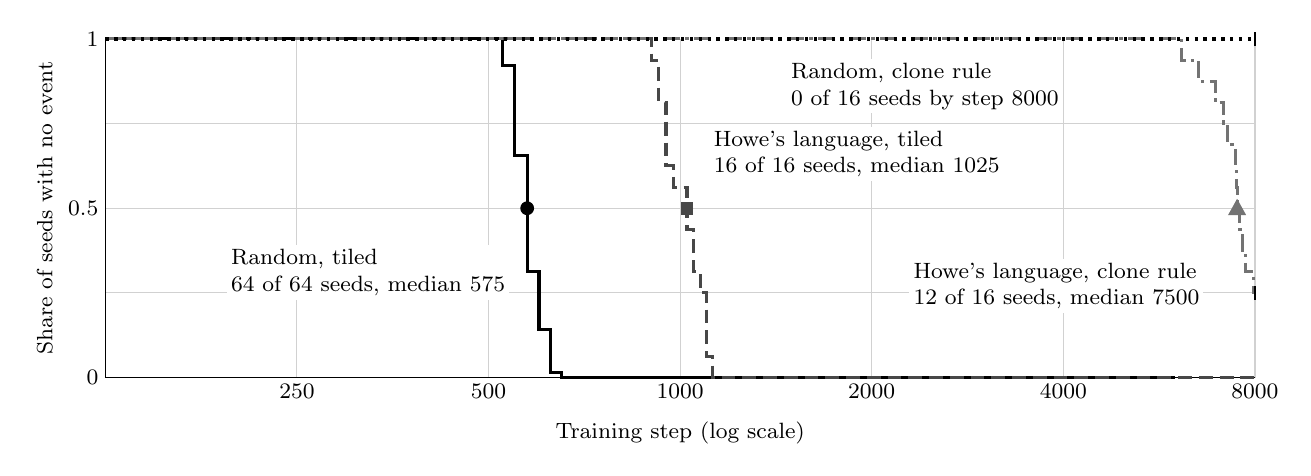
\begin{tikzpicture}
\draw[black!18, line width=0.4pt] (0.000,1.075) -- (14.600,1.075);
\draw[black!18, line width=0.4pt] (0.000,2.150) -- (14.600,2.150);
\draw[black!18, line width=0.4pt] (0.000,3.225) -- (14.600,3.225);
\draw[black!18, line width=0.4pt] (2.433,0.000) -- (2.433,4.300);
\node[anchor=north, inner sep=1.5pt, align=left, font=\footnotesize] at (2.433,-0.030) {250};
\draw[black!18, line width=0.4pt] (4.867,0.000) -- (4.867,4.300);
\node[anchor=north, inner sep=1.5pt, align=left, font=\footnotesize] at (4.867,-0.030) {500};
\draw[black!18, line width=0.4pt] (7.300,0.000) -- (7.300,4.300);
\node[anchor=north, inner sep=1.5pt, align=left, font=\footnotesize] at (7.300,-0.030) {1000};
\draw[black!18, line width=0.4pt] (9.733,0.000) -- (9.733,4.300);
\node[anchor=north, inner sep=1.5pt, align=left, font=\footnotesize] at (9.733,-0.030) {2000};
\draw[black!18, line width=0.4pt] (12.167,0.000) -- (12.167,4.300);
\node[anchor=north, inner sep=1.5pt, align=left, font=\footnotesize] at (12.167,-0.030) {4000};
\draw[black!18, line width=0.4pt] (14.600,0.000) -- (14.600,4.300);
\node[anchor=north, inner sep=1.5pt, align=left, font=\footnotesize] at (14.600,-0.030) {8000};
\draw[black, line width=0.5pt] (0.000,4.300) -- (0.000,0.000) -- (14.600,0.000);
\node[anchor=east, inner sep=1.5pt, align=left, font=\footnotesize] at (-0.030,0.000) {0};
\node[anchor=east, inner sep=1.5pt, align=left, font=\footnotesize] at (-0.030,2.150) {0.5};
\node[anchor=east, inner sep=1.5pt, align=left, font=\footnotesize] at (-0.030,4.300) {1};
\node[anchor=north, inner sep=1.5pt, align=left, font=\footnotesize] at (7.300,-0.500) {Training step (log scale)};
\node[rotate=90, anchor=south, font=\footnotesize] at (-0.55,2.150) {Share of seeds with no event};
\draw[black, line width=1.1pt] (0.000,4.300) -- (5.038,4.300) -- (5.038,4.233) -- (5.038,4.233) -- (5.038,4.166) -- (5.038,4.166) -- (5.038,4.098) -- (5.038,4.098) -- (5.038,4.031) -- (5.038,4.031) -- (5.038,3.964) -- (5.201,3.964) -- (5.201,3.897) -- (5.201,3.897) -- (5.201,3.830) -- (5.201,3.830) -- (5.201,3.762) -- (5.201,3.762) -- (5.201,3.695) -- (5.201,3.695) -- (5.201,3.628) -- (5.201,3.628) -- (5.201,3.561) -- (5.201,3.561) -- (5.201,3.494) -- (5.201,3.494) -- (5.201,3.427) -- (5.201,3.427) -- (5.201,3.359) -- (5.201,3.359) -- (5.201,3.292) -- (5.201,3.292) -- (5.201,3.225) -- (5.201,3.225) -- (5.201,3.158) -- (5.201,3.158) -- (5.201,3.091) -- (5.201,3.091) -- (5.201,3.023) -- (5.201,3.023) -- (5.201,2.956) -- (5.201,2.956) -- (5.201,2.889) -- (5.201,2.889) -- (5.201,2.822) -- (5.357,2.822) -- (5.357,2.755) -- (5.357,2.755) -- (5.357,2.688) -- (5.357,2.688) -- (5.357,2.620) -- (5.357,2.620) -- (5.357,2.553) -- (5.357,2.553) -- (5.357,2.486) -- (5.357,2.486) -- (5.357,2.419) -- (5.357,2.419) -- (5.357,2.352) -- (5.357,2.352) -- (5.357,2.284) -- (5.357,2.284) -- (5.357,2.217) -- (5.357,2.217) -- (5.357,2.150) -- (5.357,2.150) -- (5.357,2.083) -- (5.357,2.083) -- (5.357,2.016) -- (5.357,2.016) -- (5.357,1.948) -- (5.357,1.948) -- (5.357,1.881) -- (5.357,1.881) -- (5.357,1.814) -- (5.357,1.814) -- (5.357,1.747) -- (5.357,1.747) -- (5.357,1.680) -- (5.357,1.680) -- (5.357,1.612) -- (5.357,1.612) -- (5.357,1.545) -- (5.357,1.545) -- (5.357,1.478) -- (5.357,1.478) -- (5.357,1.411) -- (5.357,1.411) -- (5.357,1.344) -- (5.507,1.344) -- (5.507,1.277) -- (5.507,1.277) -- (5.507,1.209) -- (5.507,1.209) -- (5.507,1.142) -- (5.507,1.142) -- (5.507,1.075) -- (5.507,1.075) -- (5.507,1.008) -- (5.507,1.008) -- (5.507,0.941) -- (5.507,0.941) -- (5.507,0.873) -- (5.507,0.873) -- (5.507,0.806) -- (5.507,0.806) -- (5.507,0.739) -- (5.507,0.739) -- (5.507,0.672) -- (5.507,0.672) -- (5.507,0.605) -- (5.650,0.605) -- (5.650,0.537) -- (5.650,0.537) -- (5.650,0.470) -- (5.650,0.470) -- (5.650,0.403) -- (5.650,0.403) -- (5.650,0.336) -- (5.650,0.336) -- (5.650,0.269) -- (5.650,0.269) -- (5.650,0.202) -- (5.650,0.202) -- (5.650,0.134) -- (5.650,0.134) -- (5.650,0.067) -- (5.788,0.067) -- (5.788,0.000) -- (13.590,0.000);
\draw[black, fill=black, line width=0.7pt] (5.357,2.150) circle (0.075);
\draw[black!72, line width=1.1pt, dash pattern=on 5pt off 2.5pt] (0.000,4.300) -- (6.930,4.300) -- (6.930,4.031) -- (7.026,4.031) -- (7.026,3.762) -- (7.026,3.762) -- (7.026,3.494) -- (7.120,3.494) -- (7.120,3.225) -- (7.120,3.225) -- (7.120,2.956) -- (7.120,2.956) -- (7.120,2.688) -- (7.211,2.688) -- (7.211,2.419) -- (7.387,2.419) -- (7.387,2.150) -- (7.387,2.150) -- (7.387,1.881) -- (7.471,1.881) -- (7.471,1.612) -- (7.471,1.612) -- (7.471,1.344) -- (7.554,1.344) -- (7.554,1.075) -- (7.635,1.075) -- (7.635,0.806) -- (7.635,0.806) -- (7.635,0.537) -- (7.635,0.537) -- (7.635,0.269) -- (7.713,0.269) -- (7.713,0.000) -- (14.600,0.000);
\draw[black!72, fill=black!72, line width=0.7pt] (7.319,2.082) rectangle (7.455,2.218);
\draw[black!55, line width=1.1pt, dash pattern=on 6pt off 2pt on 1.2pt off 2pt] (0.000,4.300) -- (13.662,4.300) -- (13.662,4.031) -- (13.885,4.031) -- (13.885,3.762) -- (14.093,3.762) -- (14.093,3.494) -- (14.206,3.494) -- (14.206,3.225) -- (14.254,3.225) -- (14.254,2.956) -- (14.350,2.956) -- (14.350,2.688) -- (14.362,2.688) -- (14.362,2.419) -- (14.373,2.419) -- (14.373,2.150) -- (14.408,2.150) -- (14.408,1.881) -- (14.443,1.881) -- (14.443,1.612) -- (14.477,1.612) -- (14.477,1.344) -- (14.578,1.344) -- (14.578,1.075) -- (14.600,1.075);
\draw[black, line width=0.8pt] (14.600,0.985) -- (14.600,1.165);
\draw[black!55, fill=black!55, line width=0.7pt] (14.373,2.245) -- (14.278,2.074) -- (14.468,2.074) -- cycle;
\draw[black, line width=1.2pt, dash pattern=on 1.2pt off 2pt] (0.000,4.300) -- (14.600,4.300);
\draw[black, line width=0.8pt] (14.600,4.210) -- (14.600,4.390);
\node[anchor=east, inner sep=1.5pt, align=left, font=\footnotesize, fill=white] at (5.137,1.333) {Random, tiled\\64 of 64 seeds, median 575};
\node[anchor=west, inner sep=1.5pt, align=left, font=\footnotesize, fill=white] at (7.667,2.838) {Howe's language, tiled\\16 of 16 seeds, median 1025};
\node[anchor=east, inner sep=1.5pt, align=left, font=\footnotesize, fill=white] at (13.953,1.161) {Howe's language, clone rule\\12 of 16 seeds, median 7500};
\node[anchor=east, inner sep=1.5pt, align=left, font=\footnotesize, fill=white] at (12.167,3.698) {Random, clone rule\\0 of 16 seeds by step 8000};
\end{tikzpicture}

\caption{Kaplan-Meier survival by curriculum on the \arm{2}{2} study model at lr \nLrHi. Each line is one curriculum, with \nNTwoTwoHi\ seeds for random tiled and \nNBiClone\ for each of the others, all from one budget of \nBudgetBiClone\ steps except random tiled at \nBudgetTwoTwoHi. Censored runs end at the tick on the right: \nEvBiClone\ of \nNBiClone\ fired under Howe's language with the clone rule, and \nEvUniClone\ of \nNUniClone\ for random tokens with the clone rule. A marker shows each median. No tiled run was censored.}
\label{fig:survival}
\end{figure}

\begin{table}[t]
\centering
\small
\caption{One factor changed at a time, on the study's \arm{2}{2} model at lr \nLrHi, with a budget of \nCrossedBudget\ steps. Here $p$ is the repeat probability, ``language'' is Howe's bigram language, and ``uniform'' is uniform random tokens. Arms have \nRuleBiCloneN\ seeds, except the \nNTwoTwoHi-seed main arm at periods \nRangeShort.}
\label{tab:factors}
\begin{tabular}{llll}
\toprule
Changed alone & Held fixed & One side & Other side \\
\midrule
Repeat rule & language, $p$=1, \nRangeShort & tiled, \nRuleBiTiledEv\ of \nRuleBiCloneN, median \nRuleBiTiledMed & clone, \nRuleBiCloneEv\ of \nRuleBiCloneN \\
Repeat rule & uniform, $p$=\nPRepLow, \nRangeLong & tiled, \nRuleUniTiledEv\ of \nRuleBiCloneN, median \nRuleUniTiledMed & clone, \nRuleUniCloneEv\ of \nRuleBiCloneN \\
Period range & uniform, tiled, $p$=1 & \nRangeShort, \nEvTwoTwoHi\ of \nNTwoTwoHi, median \nMedTwoTwoHi & \nRangeLong, \nRangeUniLongEv\ of \nRuleBiCloneN, median \nRangeUniLongMed \\
Period range & language, clone, $p$=\nPRepLow & \nRangeShort, \nRangeBiShortEv\ of \nRuleBiCloneN & \nRangeLong, \nRangeBiLongEv\ of \nRuleBiCloneN, median \nRangeBiLongMed \\
Repeat rate & uniform, tiled, \nRangeLong & $p$=1, \nRangeUniLongEv\ of \nRuleBiCloneN, median \nRangeUniLongMed & $p$=\nPRepLow, \nRuleUniTiledEv\ of \nRuleBiCloneN, median \nRuleUniTiledMed \\
Repeat rate & language, clone, \nRangeShort & $p$=1, \nRuleBiCloneEv\ of \nRuleBiCloneN & $p$=\nPRepLow, \nRangeBiShortEv\ of \nRuleBiCloneN \\
Language & tiled, $p$=1, \nRangeShort & uniform, \nEvTwoTwoHi\ of \nNTwoTwoHi, median \nMedTwoTwoHi & language, \nEvBiTiled\ of \nNBiTiled, median \nMedBiTiled \\
Language & clone, $p$=\nPRepLow, \nRangeLong & uniform, \nEvUniClone\ of \nNUniClone & language, \nEvBiClone\ of \nNBiClone, median \nMedBiClone \\
\bottomrule
\end{tabular}
\end{table}

The repeat rule carries most of the drop in steps. On Howe's language, tiling fires on every seed and the clone rule on \nRuleBiCloneEv\ of \nRuleBiCloneN, so the clone arm has no median by step \nCrossedBudget\ and the ratio is at least \nRuleBiBound. On uniform tokens the same bound is \nRuleUniBound. The period range changes direction between rules. Under tiling, \nRangeLong\ against \nRangeShort\ is a ratio of \nRangeUniRatio\ (\nRangeUniCi), and under the clone rule the shorter periods are the worse ones. Repeat rate is smaller, at a ratio of \nRateRatio\ (\nRateCi) for a probability of \nPRepLow\ against 1 under tiling, which the plan did not name as a contrast but which its arms contain. Language also changes direction. Under tiling it is a time ratio of \nLanguageFit\ (\nLanguageFitCi) against uniform tokens, and under the clone rule it is the only one of the two that fires.

Training on random repeats is not new. shaikabdul185-arch~\cite{shaik}, xanderchinxyz~\cite{xander} and gama~\cite{gama} do it too, and Zucchet et al.~\cite{zucchet} found that repetition can greatly speed up the emergence of sparse attention, in theory and on an in-context associative recall task. The result here is the attribution, one factor at a time, on one model. Howe's curriculum does not transfer to the tab's size in the steps a tab can spare. The tab's own model on Howe's language and clone rule fired on \nTabHoweEv\ of \nTabHoweN\ seeds by step \nTabHoweBudget. We stopped there, so this does not say it never would.

\subsection{Weight tying}

On random-repeat data, at equal depth, tying weights delayed the event. Table~\ref{tab:tying} gives both estimators at both learning rates, and Figure~\ref{fig:depth} shows the medians. The plan preregistered the censored log-normal fit, and we added the ratio of Kaplan-Meier medians after correcting the fit (Section~\ref{sec:prereg}). The two agree where every run fires. They disagree where a few runs stall, such as \arm{4}{1} at lr \nLrHi, where \nCensorFourOne\ of \nNFourOneHi\ had no event by step \nBudgetFourOneHi, because censored runs pull the fit's mean log time upward and leave the median alone. Steps are multiples of \nEvalEvery, so a Kaplan-Meier interval can touch its own point estimate.

\begin{table}[t]
\centering
\small
\caption{Time ratio of a tied arm against the untied arm of equal depth, with bootstrap 95\% intervals over seeds. Seeds per arm: \nNTwoTwoHi\ at depths 2 to 4, \nNEightTwoHi\ at depth 8, \nNTwelveFourHi\ at depth 12.}
\label{tab:tying}
\begin{tabular}{lllll}
\toprule
Contrast & \multicolumn{2}{c}{lr \nLrHi} & \multicolumn{2}{c}{lr \nLrLo} \\
 & Censored log-normal & KM medians & Censored log-normal & KM medians \\
\midrule
\arm{2}{1} / \arm{2}{2} & \nFitTwoOneVsTwoTwoHi\ (\nFitCiTwoOneVsTwoTwoHi) & \nKmTwoOneVsTwoTwoHi\ (\nKmCiTwoOneVsTwoTwoHi) & \nFitTwoOneVsTwoTwoLo\ (\nFitCiTwoOneVsTwoTwoLo) & \nKmTwoOneVsTwoTwoLo\ (\nKmCiTwoOneVsTwoTwoLo) \\
\arm{3}{1} / \arm{3}{3} & \nFitThreeOneVsThreeThreeHi\ (\nFitCiThreeOneVsThreeThreeHi) & \nKmThreeOneVsThreeThreeHi\ (\nKmCiThreeOneVsThreeThreeHi) & \nFitThreeOneVsThreeThreeLo\ (\nFitCiThreeOneVsThreeThreeLo) & \nKmThreeOneVsThreeThreeLo\ (\nKmCiThreeOneVsThreeThreeLo) \\
\arm{4}{1} / \arm{4}{4} & \nFitFourOneVsFourFourHi\ (\nFitCiFourOneVsFourFourHi) & \nKmFourOneVsFourFourHi\ (\nKmCiFourOneVsFourFourHi) & \nFitFourOneVsFourFourLo\ (\nFitCiFourOneVsFourFourLo) & \nKmFourOneVsFourFourLo\ (\nKmCiFourOneVsFourFourLo) \\
\arm{4}{2} / \arm{4}{4} & \nFitFourTwoVsFourFourHi\ (\nFitCiFourTwoVsFourFourHi) & \nKmFourTwoVsFourFourHi\ (\nKmCiFourTwoVsFourFourHi) & \nFitFourTwoVsFourFourLo\ (\nFitCiFourTwoVsFourFourLo) & \nKmFourTwoVsFourFourLo\ (\nKmCiFourTwoVsFourFourLo) \\
\arm{8}{2} / \arm{8}{8} & \nFitEightTwoVsEightEightHi\ (\nFitCiEightTwoVsEightEightHi) & \nKmEightTwoVsEightEightHi\ (\nKmCiEightTwoVsEightEightHi) & & \\
\arm{12}{4} / \arm{12}{12} & \nFitTwelveFourVsTwelveTwelveHi\ (\nFitCiTwelveFourVsTwelveTwelveHi) & \nTwelveKm\ (\nTwelveKmCi) & & \\
\bottomrule
\end{tabular}
\end{table}

\begin{figure}[t]
\centering
% Generated by paper/figures.py from results/. Do not edit.
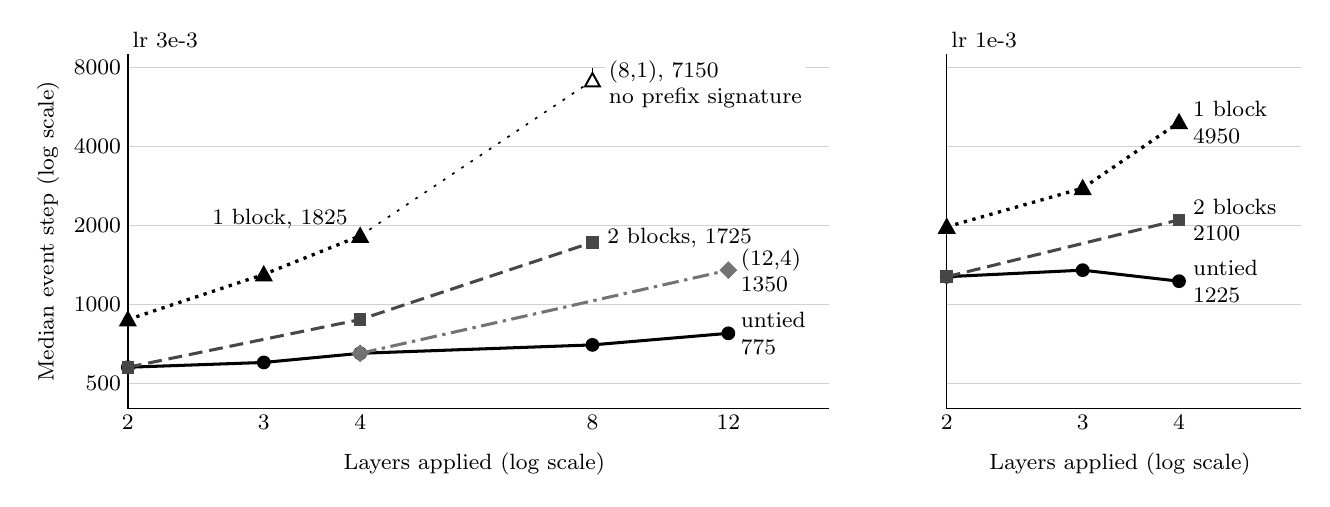
\begin{tikzpicture}
\draw[black!18, line width=0.4pt] (0.000,0.323) -- (8.900,0.323);
\draw[black!18, line width=0.4pt] (10.400,0.323) -- (14.900,0.323);
\node[anchor=east, inner sep=1.5pt, align=left, font=\footnotesize] at (-0.030,0.323) {500};
\draw[black!18, line width=0.4pt] (0.000,1.324) -- (8.900,1.324);
\draw[black!18, line width=0.4pt] (10.400,1.324) -- (14.900,1.324);
\node[anchor=east, inner sep=1.5pt, align=left, font=\footnotesize] at (-0.030,1.324) {1000};
\draw[black!18, line width=0.4pt] (0.000,2.326) -- (8.900,2.326);
\draw[black!18, line width=0.4pt] (10.400,2.326) -- (14.900,2.326);
\node[anchor=east, inner sep=1.5pt, align=left, font=\footnotesize] at (-0.030,2.326) {2000};
\draw[black!18, line width=0.4pt] (0.000,3.328) -- (8.900,3.328);
\draw[black!18, line width=0.4pt] (10.400,3.328) -- (14.900,3.328);
\node[anchor=east, inner sep=1.5pt, align=left, font=\footnotesize] at (-0.030,3.328) {4000};
\draw[black!18, line width=0.4pt] (0.000,4.330) -- (8.900,4.330);
\draw[black!18, line width=0.4pt] (10.400,4.330) -- (14.900,4.330);
\node[anchor=east, inner sep=1.5pt, align=left, font=\footnotesize] at (-0.030,4.330) {8000};
\draw[black, line width=0.5pt] (0.000,4.500) -- (0.000,0.000) -- (8.900,0.000);
\draw[black, line width=0.5pt] (10.400,4.500) -- (10.400,0.000) -- (14.900,0.000);
\node[anchor=north, inner sep=1.5pt, align=left, font=\footnotesize] at (0.000,-0.030) {2};
\node[anchor=north, inner sep=1.5pt, align=left, font=\footnotesize] at (1.726,-0.030) {3};
\node[anchor=north, inner sep=1.5pt, align=left, font=\footnotesize] at (2.950,-0.030) {4};
\node[anchor=north, inner sep=1.5pt, align=left, font=\footnotesize] at (5.900,-0.030) {8};
\node[anchor=north, inner sep=1.5pt, align=left, font=\footnotesize] at (7.626,-0.030) {12};
\node[anchor=north, inner sep=1.5pt, align=left, font=\footnotesize] at (10.400,-0.030) {2};
\node[anchor=north, inner sep=1.5pt, align=left, font=\footnotesize] at (12.126,-0.030) {3};
\node[anchor=north, inner sep=1.5pt, align=left, font=\footnotesize] at (13.350,-0.030) {4};
\node[anchor=north, inner sep=1.5pt, align=left, font=\footnotesize] at (4.400,-0.500) {Layers applied (log scale)};
\node[anchor=north, inner sep=1.5pt, align=left, font=\footnotesize] at (12.600,-0.500) {Layers applied (log scale)};
\node[anchor=south west, inner sep=1.5pt, align=left, font=\footnotesize] at (0.000,4.530) {lr 3e-3};
\node[anchor=south west, inner sep=1.5pt, align=left, font=\footnotesize] at (10.400,4.530) {lr 1e-3};
\node[rotate=90, anchor=south, font=\footnotesize] at (-0.75,2.250) {Median event step (log scale)};
\draw[black, line width=1.1pt] (0.000,0.525) -- (1.726,0.586) -- (2.950,0.702) -- (5.900,0.809) -- (7.626,0.956);
\draw[black, line width=0.5pt] (0.000,0.525) -- (0.000,0.525);
\draw[black, fill=black, line width=0.7pt] (0.000,0.525) circle (0.075);
\draw[black, line width=0.5pt] (1.726,0.586) -- (1.726,0.645);
\draw[black, fill=black, line width=0.7pt] (1.726,0.586) circle (0.075);
\draw[black, line width=0.5pt] (2.950,0.702) -- (2.950,0.702);
\draw[black, fill=black, line width=0.7pt] (2.950,0.702) circle (0.075);
\draw[black, line width=0.5pt] (5.900,0.809) -- (5.900,0.860);
\draw[black, fill=black, line width=0.7pt] (5.900,0.809) circle (0.075);
\draw[black, line width=0.5pt] (7.626,0.909) -- (7.626,1.002);
\draw[black, fill=black, line width=0.7pt] (7.626,0.956) circle (0.075);
\draw[black!72, line width=1.1pt, dash pattern=on 5pt off 2.5pt] (0.000,0.525) -- (2.950,1.131) -- (5.900,2.112);
\draw[black!72, line width=0.5pt] (0.000,0.525) -- (0.000,0.525);
\draw[black!72, fill=black!72, line width=0.7pt] (-0.068,0.457) rectangle (0.068,0.593);
\draw[black!72, line width=0.5pt] (2.950,1.089) -- (2.950,1.131);
\draw[black!72, fill=black!72, line width=0.7pt] (2.882,1.063) rectangle (3.018,1.199);
\draw[black!72, line width=0.5pt] (5.900,2.048) -- (5.900,2.112);
\draw[black!72, fill=black!72, line width=0.7pt] (5.832,2.044) rectangle (5.968,2.180);
\draw[black, line width=1.2pt, dash pattern=on 1.2pt off 2pt] (0.000,1.131) -- (1.726,1.704) -- (2.950,2.194);
\draw[black, line width=0.5pt] (0.000,1.131) -- (0.000,1.172);
\draw[black, fill=black, line width=0.7pt] (0.000,1.226) -- (-0.095,1.055) -- (0.095,1.055) -- cycle;
\draw[black, line width=0.5pt] (1.726,1.618) -- (1.726,1.731);
\draw[black, fill=black, line width=0.7pt] (1.726,1.799) -- (1.631,1.628) -- (1.821,1.628) -- cycle;
\draw[black, line width=0.5pt] (2.950,2.133) -- (2.950,2.271);
\draw[black, fill=black, line width=0.7pt] (2.950,2.289) -- (2.855,2.118) -- (3.045,2.118) -- cycle;
\draw[black!55, line width=1.1pt, dash pattern=on 6pt off 2pt on 1.2pt off 2pt] (2.950,0.702) -- (7.626,1.758);
\draw[black!55, line width=0.5pt] (2.950,0.702) -- (2.950,0.702);
\draw[black!55, fill=black!55, line width=0.7pt] (2.950,0.797) -- (2.855,0.702) -- (2.950,0.607) -- (3.045,0.702) -- cycle;
\draw[black!55, line width=0.5pt] (7.626,1.704) -- (7.626,1.811);
\draw[black!55, fill=black!55, line width=0.7pt] (7.626,1.853) -- (7.531,1.758) -- (7.626,1.663) -- (7.721,1.758) -- cycle;
\draw[black, line width=0.6pt, dash pattern=on 1pt off 3pt] (2.950,2.194) -- (5.900,4.167);
\draw[black, line width=0.5pt] (5.900,4.095) -- (5.900,4.330);
\draw[black, fill=white, line width=0.7pt] (5.900,4.262) -- (5.805,4.091) -- (5.995,4.091) -- cycle;
\node[anchor=west, inner sep=1.5pt, align=left, font=\footnotesize] at (7.726,0.956) {untied\\775};
\node[anchor=west, inner sep=1.5pt, align=left, font=\footnotesize] at (6.030,2.172) {2 blocks, 1725};
\node[anchor=east, inner sep=1.5pt, align=left, font=\footnotesize] at (2.850,2.414) {1 block, 1825};
\node[anchor=west, inner sep=1.5pt, align=left, font=\footnotesize, fill=white] at (6.050,4.117) {(8,1), 7150\\no prefix signature};
\node[anchor=west, inner sep=1.5pt, align=left, font=\footnotesize] at (7.726,1.758) {(12,4)\\1350};
\draw[black, line width=1.1pt] (10.400,1.675) -- (12.126,1.758) -- (13.350,1.618);
\draw[black, line width=0.5pt] (10.400,1.647) -- (10.400,1.704);
\draw[black, fill=black, line width=0.7pt] (10.400,1.675) circle (0.075);
\draw[black, line width=0.5pt] (12.126,1.731) -- (12.126,1.759);
\draw[black, fill=black, line width=0.7pt] (12.126,1.758) circle (0.075);
\draw[black, line width=0.5pt] (13.350,1.588) -- (13.350,1.647);
\draw[black, fill=black, line width=0.7pt] (13.350,1.618) circle (0.075);
\draw[black!72, line width=1.1pt, dash pattern=on 5pt off 2.5pt] (10.400,1.675) -- (13.350,2.397);
\draw[black!72, line width=0.5pt] (10.400,1.647) -- (10.400,1.704);
\draw[black!72, fill=black!72, line width=0.7pt] (10.332,1.607) rectangle (10.468,1.743);
\draw[black!72, line width=0.5pt] (13.350,2.362) -- (13.350,2.414);
\draw[black!72, fill=black!72, line width=0.7pt] (13.282,2.329) rectangle (13.418,2.465);
\draw[black, line width=1.2pt, dash pattern=on 1.2pt off 2pt] (10.400,2.308) -- (12.126,2.799) -- (13.350,3.636);
\draw[black, line width=0.5pt] (10.400,2.271) -- (10.400,2.326);
\draw[black, fill=black, line width=0.7pt] (10.400,2.403) -- (10.305,2.232) -- (10.495,2.232) -- cycle;
\draw[black, line width=0.5pt] (12.126,2.773) -- (12.126,2.863);
\draw[black, fill=black, line width=0.7pt] (12.126,2.894) -- (12.031,2.723) -- (12.221,2.723) -- cycle;
\draw[black, line width=0.5pt] (13.350,3.606) -- (13.350,3.700);
\draw[black, fill=black, line width=0.7pt] (13.350,3.731) -- (13.255,3.560) -- (13.445,3.560) -- cycle;
\node[anchor=west, inner sep=1.5pt, align=left, font=\footnotesize] at (13.470,1.618) {untied\\1225};
\node[anchor=west, inner sep=1.5pt, align=left, font=\footnotesize] at (13.470,2.397) {2 blocks\\2100};
\node[anchor=west, inner sep=1.5pt, align=left, font=\footnotesize] at (13.470,3.636) {1 block\\4950};
\end{tikzpicture}

\caption{Median event step against depth and block count, with Kaplan-Meier 95\% intervals. Lines join arms with the same block count, and the solid line joins the untied arms. Each point is one arm with \nNTwoTwoHi\ seeds at depths 2 to 4, \nNEightTwoHi\ at \arm{8}{2} and \arm{8}{8}, \nNTwelveFourHi\ at depth 12, and \nNEightOneHi\ at \arm{8}{1}. Censored runs: \nCensorThreeOne\ of \nNThreeOneHi\ for \arm{3}{1} and \nCensorFourOne\ of \nNFourOneHi\ for \arm{4}{1}, both at lr \nLrHi\ and step \nBudgetFourOneHi, and no other arm shown. The open triangle is \arm{8}{1}, run to step \nBudgetEightOneHi, whose earlier \nEightOneEarlierSeeds\ seeds had \nEightOneEarlierEvents\ events by step \nEightOneEarlierBudget\ and are not merged into it.}
\label{fig:depth}
\end{figure}

The design separates tying from depth. The \arm{4}{2} arm has the unique parameters of \arm{2}{2} and the depth of \arm{4}{4}. Against \arm{4}{4} it is \nFitFourTwoVsFourFourHi\ at lr \nLrHi\ and \nFitFourTwoVsFourFourLo\ at lr \nLrLo, and against \arm{2}{2} it is \nFitFourTwoVsTwoTwoHi\ and \nFitFourTwoVsTwoTwoLo. Untied depth is nearly free in steps. Arm \arm{4}{4} against \arm{2}{2} is \nFitFourFourVsTwoTwoHi\ at lr \nLrHi\ and \nFitFourFourVsTwoTwoLo\ at lr \nLrLo, and \arm{8}{8} against \arm{4}{4} is \nFitEightEightVsFourFourHi. Each step costs more, so in floating point operations \arm{8}{8} against \arm{4}{4} is \nFlopEightEightVsFourFourHi.

There is no crossover at these depths. The second plan said a crossover would be claimed only if a looped arm's interval lay wholly below 1, and the lowest bound across the tying contrasts in Table~\ref{tab:tying} is \nLowestTyingBound. Arm \arm{8}{1} is its own case. Its first \nEightOneEarlierSeeds\ seeds had no event by step \nEightOneEarlierBudget, which bounds its ratio against \arm{8}{8} at no less than \nEightOneBound. The third plan then ran \nNEightOneHi\ seeds to step \nBudgetEightOneHi, and \nEvEightOneHi\ of \nNEightOneHi\ fire at a median of step \nMedEightOneHi, a time ratio of \nFitEightOneVsEightEightHi\ (\nFitCiEightOneVsEightEightHi). We keep that arm out of the tying claim, because it shows no prefix signature (Section~\ref{sec:exploratory}).

We did not find this delay reported within our coverage. The closest work finds looped models earlier than a dense model, on other tasks and at greater depth, and we do not claim a contradiction. Kapl et al.~\cite{kapl} find in-context accuracy emerging earlier for looped models than for a 12-layer dense one, on Omniglot-based tasks. Sesodia et al.~\cite{sesodia} report a $4\times8$ looped model reaching the solution sooner than an untied 32-layer model at a lower learning rate (\nSoonerLooped\ training steps against \nSoonerUntied), on depth-bound algorithmic tasks. The task here is copying random repeats, the models have 2 to 12 layers, and the measure is Howe's event.

We did not separate effective step size from structure. A tied block's gradient sums across its passes, Adam rescales each parameter by its running gradient magnitude, and lowering lr from \nLrHi\ to \nLrLo\ slowed looped arms further, \arm{4}{1} from \nMedFourOneHi\ to \nMedFourOneLo. No arm scales lr with pass count. So this is a delay at these depths, learning rates and data, and we do not generalize it to tying slowing learning.

\section{The forecast}
\label{sec:forecast}

Howe's law puts the anchor at a steady fraction of the time to the event. Figure~\ref{fig:gap} shows the fraction across every arm with events. Across the \nShallowArms\ uniform tiled arms at depths 2 to 4 the median runs from \nGapShallowLow\ to \nGapShallowHigh. The first plan's falsifier was an arm whose median falls outside Howe's envelope, and it fired for \nArmsOutside\ arms just under it: \arm{2}{2} at lr \nLrHi\ (\nGapTwoTwoHi), \arm{3}{3} at lr \nLrHi\ (\nGapThreeThreeHi) and \arm{2}{2} at lr \nLrLo\ (\nGapTwoTwoLo). The tab's own model at \nEvalEvery-step evals reads \nTabGap, just inside.

\begin{figure}[t]
\centering
% Generated by paper/figures.py from results/. Do not edit.
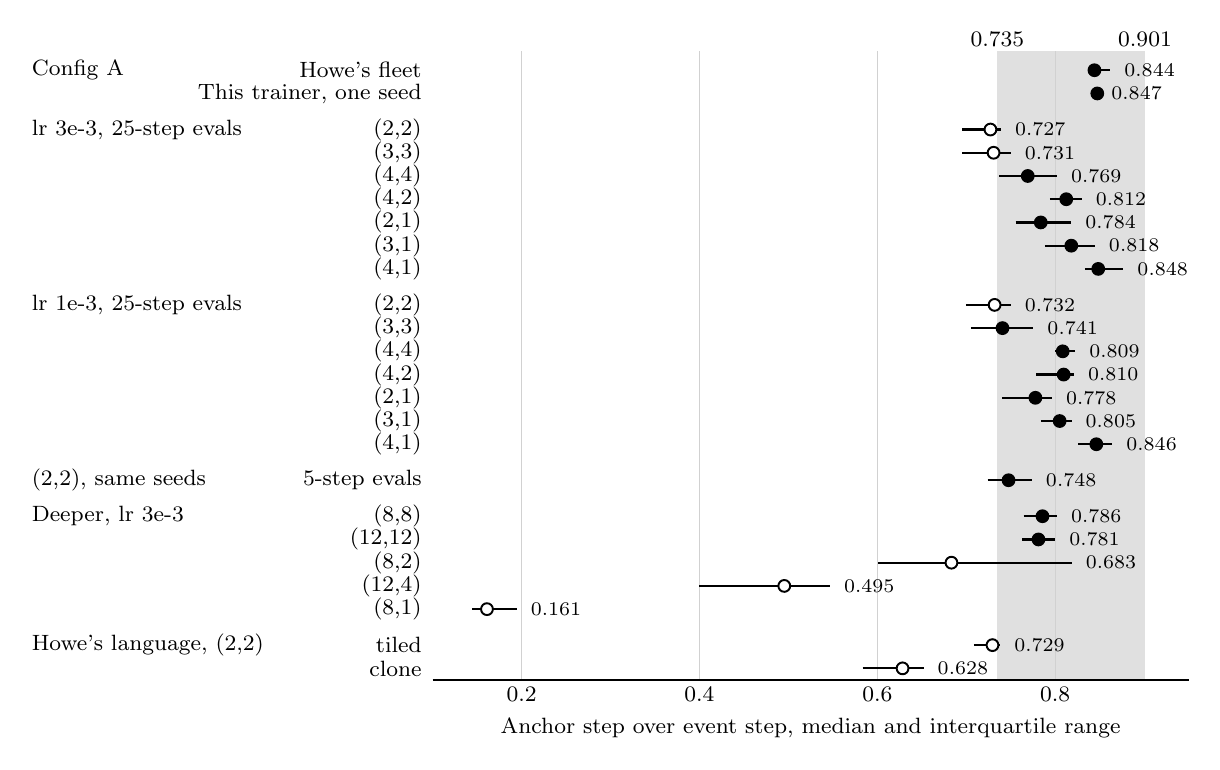
\begin{tikzpicture}
\fill[black!12] (12.322,0) rectangle (14.197,7.991);
\draw[black!18, line width=0.4pt] (6.279,0.000) -- (6.279,7.991);
\node[anchor=north, inner sep=1.5pt, align=left, font=\footnotesize] at (6.279,-0.030) {0.2};
\draw[black!18, line width=0.4pt] (8.538,0.000) -- (8.538,7.991);
\node[anchor=north, inner sep=1.5pt, align=left, font=\footnotesize] at (8.538,-0.030) {0.4};
\draw[black!18, line width=0.4pt] (10.797,0.000) -- (10.797,7.991);
\node[anchor=north, inner sep=1.5pt, align=left, font=\footnotesize] at (10.797,-0.030) {0.6};
\draw[black!18, line width=0.4pt] (13.056,0.000) -- (13.056,7.991);
\node[anchor=north, inner sep=1.5pt, align=left, font=\footnotesize] at (13.056,-0.030) {0.8};
\draw[black, line width=0.5pt] (5.150,0.000) -- (14.750,0.000);
\node[anchor=north, inner sep=1.5pt, align=left, font=\footnotesize] at (9.950,-0.420) {Anchor step over event step, median and interquartile range};
\node[anchor=south, inner sep=1.5pt, align=left, font=\footnotesize] at (12.322,7.991) {0.735};
\node[anchor=south, inner sep=1.5pt, align=left, font=\footnotesize] at (14.197,7.991) {0.901};
\node[anchor=west, inner sep=1.5pt, align=left, font=\footnotesize] at (0.000,7.744) {Config A};
\node[anchor=east, inner sep=1.5pt, align=left, font=\footnotesize] at (5.070,7.744) {Howe's fleet};
\draw[black, line width=0.8pt] (13.477,7.744) -- (13.756,7.744);
\draw[black, fill=black, line width=0.7pt] (13.555,7.744) circle (0.075);
\node[anchor=west, inner sep=1.5pt, align=left, font=\scriptsize] at (13.876,7.744) {0.844};
\node[anchor=east, inner sep=1.5pt, align=left, font=\footnotesize] at (5.070,7.449) {This trainer, one seed};
\draw[black, fill=black, line width=0.7pt] (13.591,7.449) circle (0.075);
\node[anchor=west, inner sep=1.5pt, align=left, font=\scriptsize] at (13.711,7.449) {0.847};
\node[anchor=west, inner sep=1.5pt, align=left, font=\footnotesize] at (0.000,6.991) {lr 3e-3, 25-step evals};
\node[anchor=east, inner sep=1.5pt, align=left, font=\footnotesize] at (5.070,6.991) {(2,2)};
\draw[black, line width=0.8pt] (11.877,6.991) -- (12.368,6.991);
\draw[black, fill=white, line width=0.7pt] (12.234,6.991) circle (0.075);
\node[anchor=west, inner sep=1.5pt, align=left, font=\scriptsize] at (12.488,6.991) {0.727};
\node[anchor=east, inner sep=1.5pt, align=left, font=\footnotesize] at (5.070,6.696) {(3,3)};
\draw[black, line width=0.8pt] (11.877,6.696) -- (12.491,6.696);
\draw[black, fill=white, line width=0.7pt] (12.274,6.696) circle (0.075);
\node[anchor=west, inner sep=1.5pt, align=left, font=\scriptsize] at (12.611,6.696) {0.731};
\node[anchor=east, inner sep=1.5pt, align=left, font=\footnotesize] at (5.070,6.401) {(4,4)};
\draw[black, line width=0.8pt] (12.345,6.401) -- (13.078,6.401);
\draw[black, fill=black, line width=0.7pt] (12.708,6.401) circle (0.075);
\node[anchor=west, inner sep=1.5pt, align=left, font=\scriptsize] at (13.198,6.401) {0.769};
\node[anchor=east, inner sep=1.5pt, align=left, font=\footnotesize] at (5.070,6.106) {(4,2)};
\draw[black, line width=0.8pt] (12.989,6.106) -- (13.392,6.106);
\draw[black, fill=black, line width=0.7pt] (13.197,6.106) circle (0.075);
\node[anchor=west, inner sep=1.5pt, align=left, font=\scriptsize] at (13.512,6.106) {0.812};
\node[anchor=east, inner sep=1.5pt, align=left, font=\footnotesize] at (5.070,5.811) {(2,1)};
\draw[black, line width=0.8pt] (12.555,5.811) -- (13.261,5.811);
\draw[black, fill=black, line width=0.7pt] (12.873,5.811) circle (0.075);
\node[anchor=west, inner sep=1.5pt, align=left, font=\scriptsize] at (13.381,5.811) {0.784};
\node[anchor=east, inner sep=1.5pt, align=left, font=\footnotesize] at (5.070,5.516) {(3,1)};
\draw[black, line width=0.8pt] (12.926,5.516) -- (13.560,5.516);
\draw[black, fill=black, line width=0.7pt] (13.261,5.516) circle (0.075);
\node[anchor=west, inner sep=1.5pt, align=left, font=\scriptsize] at (13.680,5.516) {0.818};
\node[anchor=east, inner sep=1.5pt, align=left, font=\footnotesize] at (5.070,5.221) {(4,1)};
\draw[black, line width=0.8pt] (13.432,5.221) -- (13.922,5.221);
\draw[black, fill=black, line width=0.7pt] (13.603,5.221) circle (0.075);
\node[anchor=west, inner sep=1.5pt, align=left, font=\scriptsize] at (14.042,5.221) {0.848};
\node[anchor=west, inner sep=1.5pt, align=left, font=\footnotesize] at (0.000,4.764) {lr 1e-3, 25-step evals};
\node[anchor=east, inner sep=1.5pt, align=left, font=\footnotesize] at (5.070,4.764) {(2,2)};
\draw[black, line width=0.8pt] (11.921,4.764) -- (12.491,4.764);
\draw[black, fill=white, line width=0.7pt] (12.287,4.764) circle (0.075);
\node[anchor=west, inner sep=1.5pt, align=left, font=\scriptsize] at (12.611,4.764) {0.732};
\node[anchor=east, inner sep=1.5pt, align=left, font=\footnotesize] at (5.070,4.469) {(3,3)};
\draw[black, line width=0.8pt] (11.987,4.469) -- (12.779,4.469);
\draw[black, fill=black, line width=0.7pt] (12.387,4.469) circle (0.075);
\node[anchor=west, inner sep=1.5pt, align=left, font=\scriptsize] at (12.899,4.469) {0.741};
\node[anchor=east, inner sep=1.5pt, align=left, font=\footnotesize] at (5.070,4.174) {(4,4)};
\draw[black, line width=0.8pt] (13.056,4.174) -- (13.311,4.174);
\draw[black, fill=black, line width=0.7pt] (13.152,4.174) circle (0.075);
\node[anchor=west, inner sep=1.5pt, align=left, font=\scriptsize] at (13.431,4.174) {0.809};
\node[anchor=east, inner sep=1.5pt, align=left, font=\footnotesize] at (5.070,3.879) {(4,2)};
\draw[black, line width=0.8pt] (12.816,3.879) -- (13.295,3.879);
\draw[black, fill=black, line width=0.7pt] (13.164,3.879) circle (0.075);
\node[anchor=west, inner sep=1.5pt, align=left, font=\scriptsize] at (13.415,3.879) {0.810};
\node[anchor=east, inner sep=1.5pt, align=left, font=\footnotesize] at (5.070,3.584) {(2,1)};
\draw[black, line width=0.8pt] (12.385,3.584) -- (13.015,3.584);
\draw[black, fill=black, line width=0.7pt] (12.805,3.584) circle (0.075);
\node[anchor=west, inner sep=1.5pt, align=left, font=\scriptsize] at (13.135,3.584) {0.778};
\node[anchor=east, inner sep=1.5pt, align=left, font=\footnotesize] at (5.070,3.289) {(3,1)};
\draw[black, line width=0.8pt] (12.876,3.289) -- (13.264,3.289);
\draw[black, fill=black, line width=0.7pt] (13.113,3.289) circle (0.075);
\node[anchor=west, inner sep=1.5pt, align=left, font=\scriptsize] at (13.384,3.289) {0.805};
\node[anchor=east, inner sep=1.5pt, align=left, font=\footnotesize] at (5.070,2.994) {(4,1)};
\draw[black, line width=0.8pt] (13.347,2.994) -- (13.781,2.994);
\draw[black, fill=black, line width=0.7pt] (13.579,2.994) circle (0.075);
\node[anchor=west, inner sep=1.5pt, align=left, font=\scriptsize] at (13.901,2.994) {0.846};
\node[anchor=west, inner sep=1.5pt, align=left, font=\footnotesize] at (0.000,2.537) {(2,2), same seeds};
\node[anchor=east, inner sep=1.5pt, align=left, font=\footnotesize] at (5.070,2.537) {5-step evals};
\draw[black, line width=0.8pt] (12.197,2.537) -- (12.760,2.537);
\draw[black, fill=black, line width=0.7pt] (12.464,2.537) circle (0.075);
\node[anchor=west, inner sep=1.5pt, align=left, font=\scriptsize] at (12.880,2.537) {0.748};
\node[anchor=west, inner sep=1.5pt, align=left, font=\footnotesize] at (0.000,2.080) {Deeper, lr 3e-3};
\node[anchor=east, inner sep=1.5pt, align=left, font=\footnotesize] at (5.070,2.080) {(8,8)};
\draw[black, line width=0.8pt] (12.657,2.080) -- (13.078,2.080);
\draw[black, fill=black, line width=0.7pt] (12.895,2.080) circle (0.075);
\node[anchor=west, inner sep=1.5pt, align=left, font=\scriptsize] at (13.198,2.080) {0.786};
\node[anchor=east, inner sep=1.5pt, align=left, font=\footnotesize] at (5.070,1.785) {(12,12)};
\draw[black, line width=0.8pt] (12.637,1.785) -- (13.056,1.785);
\draw[black, fill=black, line width=0.7pt] (12.844,1.785) circle (0.075);
\node[anchor=west, inner sep=1.5pt, align=left, font=\scriptsize] at (13.176,1.785) {0.781};
\node[anchor=east, inner sep=1.5pt, align=left, font=\footnotesize] at (5.070,1.490) {(8,2)};
\draw[black, line width=0.8pt] (10.807,1.490) -- (13.265,1.490);
\draw[black, fill=white, line width=0.7pt] (11.739,1.490) circle (0.075);
\node[anchor=west, inner sep=1.5pt, align=left, font=\scriptsize] at (13.385,1.490) {0.683};
\node[anchor=east, inner sep=1.5pt, align=left, font=\footnotesize] at (5.070,1.195) {(12,4)};
\draw[black, line width=0.8pt] (8.538,1.195) -- (10.195,1.195);
\draw[black, fill=white, line width=0.7pt] (9.616,1.195) circle (0.075);
\node[anchor=west, inner sep=1.5pt, align=left, font=\scriptsize] at (10.315,1.195) {0.495};
\node[anchor=east, inner sep=1.5pt, align=left, font=\footnotesize] at (5.070,0.900) {(8,1)};
\draw[black, line width=0.8pt] (5.655,0.900) -- (6.217,0.900);
\draw[black, fill=white, line width=0.7pt] (5.840,0.900) circle (0.075);
\node[anchor=west, inner sep=1.5pt, align=left, font=\scriptsize] at (6.337,0.900) {0.161};
\node[anchor=west, inner sep=1.5pt, align=left, font=\footnotesize] at (0.000,0.443) {Howe's language, (2,2)};
\node[anchor=east, inner sep=1.5pt, align=left, font=\footnotesize] at (5.070,0.443) {tiled};
\draw[black, line width=0.8pt] (12.023,0.443) -- (12.357,0.443);
\draw[black, fill=white, line width=0.7pt] (12.260,0.443) circle (0.075);
\node[anchor=west, inner sep=1.5pt, align=left, font=\scriptsize] at (12.477,0.443) {0.729};
\node[anchor=east, inner sep=1.5pt, align=left, font=\footnotesize] at (5.070,0.148) {clone};
\draw[black, line width=0.8pt] (10.612,0.148) -- (11.385,0.148);
\draw[black, fill=white, line width=0.7pt] (11.118,0.148) circle (0.075);
\node[anchor=west, inner sep=1.5pt, align=left, font=\scriptsize] at (11.505,0.148) {0.628};
\end{tikzpicture}

\caption{Anchor fraction by arm against Howe's frozen envelope (shaded). Filled markers lie inside the envelope and open markers outside. Seeds per arm: \nHoweSeeds\ for Howe's fleet, 1 for this trainer at config A, \nNTwoTwoHi\ at depths 2 to 4, \nSpacingSeeds\ for the same-seed rerun, \nNEightEightHi\ at \arm{8}{8} and \arm{8}{2}, \nNTwelveFourHi\ at depth 12, \nNEightOneHi\ at \arm{8}{1}, and \nNBiClone\ for each other curriculum. Fractions count only runs where both the event and the anchor fired, so \nCensorThreeOne\ censored runs of \arm{3}{1} and \nCensorFourOne\ of \arm{4}{1} at lr \nLrHi, \nAnchorMissArm\ anchor misses of \arm{3}{3} at lr \nLrLo, and the \nCloneCensored\ censored runs of the clone arm are not in them. Random tokens with the clone rule had no events and do not appear.}
\label{fig:gap}
\end{figure}

The second plan predicted that the anchor's distance from chance caused the miss. A flat \nAnchorThreshold\ is \nMultHigh\ times the baseline on Howe's probe and \nMultLow\ times it on ours, so it fires earlier here. The plan ran \arm{2}{2} and \arm{2}{1} at T=\nStudyT\ and T=\nPlanTwoT, seeds \nPlanTwoSeedLow\ to \nPlanTwoSeedHigh, at \nEvalFine-step evals, under the flat anchor and under a rescaled anchor of \nMultHigh\ $b(T)$. It passes only if every arm's median under the rescaled anchor lies inside the envelope. Table~\ref{tab:anchor} shows that \arm{2}{1} at T=\nStudyT\ reads \nAncRescaledSixtyFourOne\ against \nEnvHigh, with an interval of \nAncMissCi, so the prediction failed literally on one arm. At T=\nPlanTwoT\ both arms sit inside under either anchor.

\begin{table}[t]
\centering
\small
\caption{The second plan's anchor test, \nAncRunsSixtyFourTwo\ seeds per arm. The event budget was \nPlanTwoBudget\ steps, and the fractions count seeds that fired. The envelope is \nEnvLow\ to \nEnvHigh.}
\label{tab:anchor}
\begin{tabular}{lrrrr}
\toprule
Arm & Events & Flat anchor, \nEvalFine-step & Flat anchor, \nEvalEvery-step & Rescaled, \nEvalFine-step \\
\midrule
\arm{2}{2}, T=\nStudyT & \nAncEventsSixtyFourTwo & \nAncFineSixtyFourTwo & \nAncCoarseSixtyFourTwo & \nAncRescaledSixtyFourTwo \\
\arm{2}{1}, T=\nStudyT & \nAncEventsSixtyFourOne & \nAncFineSixtyFourOne & \nAncCoarseSixtyFourOne & \nAncRescaledSixtyFourOne \\
\arm{2}{2}, T=\nPlanTwoT & \nAncEventsOneTwentyEightTwo & \nAncFineOneTwentyEightTwo & \nAncCoarseOneTwentyEightTwo & \nAncRescaledOneTwentyEightTwo \\
\arm{2}{1}, T=\nPlanTwoT & \nAncEventsOneTwentyEightOne & \nAncFineOneTwentyEightOne & \nAncCoarseOneTwentyEightOne & \nAncRescaledOneTwentyEightOne \\
\bottomrule
\end{tabular}
\end{table}

The same table pointed at eval spacing, since the flat anchor on \arm{2}{2} at T=\nStudyT\ moves from \nAncCoarseSixtyFourTwo\ to \nAncFineSixtyFourTwo\ with finer evals, on other seeds than the study's. The third plan tested this on the study's own seeds. It reran \arm{2}{2} at lr \nLrHi, seeds 1 to \nFineRuns, at \nEvalFine-step evals, continuing past the event. Reading those runs every \nEvalEvery\ steps reproduces the study's event and anchor on \nSpacingSameEvent\ of \nSpacingSeeds\ readable seeds, and \nSpacingStopped\ seeds stopped before the coarse event and are out of the comparison. On those seeds the fraction is \nGapFine\ at \nEvalFine-step evals against \nGapCoarse\ at \nEvalEvery-step, a paired median difference of \nGapDiff, and the share of seeds inside the envelope moves from \nShareCoarse\ to \nShareFine\ percent. So eval spacing explains part of the miss on that arm, and enough to move its median inside. The other two arms were not rerun at \nEvalFine-step evals.

Spacing does not explain what is left. Howe's curriculum on the small model reads \nGapBiClone, \arm{8}{2} reads \nGapEightTwoHi, and the deepest tied arms sit lower, \arm{12}{4} at \nGapTwelveFourHi\ and \arm{8}{1} at \nGapEightOneHi. A \nEvalEvery-step grid moves the fraction of a run the length of \arm{12}{4} by about \nQuantTwelve, so it cannot reach those. The untied deep arms stay inside, \arm{8}{8} at \nGapEightEightHi\ and \arm{12}{12} at \nGapTwelveTwelveHi. The within-arm rank correlation of anchor and event also moves, from \nRhoFourOneHi\ at \arm{4}{1} and lr \nLrHi\ to \nRhoTwoTwoHi\ at \arm{2}{2} and \nRhoTwelveFourHi\ at \arm{12}{4}, against Howe's \nHoweRho\ on the fleet. These gaps stay open. We report them and do not explain them.

\section{Exploratory reads}
\label{sec:exploratory}

These were not preregistered as tests, and they carry no explanation beyond the measurement.

\paragraph{Copying without the prefix signature.} At \arm{8}{1} every run crosses the event, with a copy advantage of \nEightOneMinCopy\ to \nEightOneMaxCopy\ at that step, and the top prefix score across all heads and layers there reads \nEightOneMinPrefix\ to \nEightOneMaxPrefix. Every other arm in every run file reads at least \nOtherPrefixMin. So that arm copies by a route the prefix score does not see, and the event alone does not show an induction head there. This is \nNEightOneHi\ seeds, and we do not explain it here.

\paragraph{Heads in a one-block model.} In \arm{2}{1} trained for \nHeadSteps\ steps, \nHeadBothMin\ or \nHeadBothMax\ of 4 heads score \nAnchorThreshold\ or above as previous-token heads on pass 0 and as induction heads on pass 1, on all \nHeadSeeds\ seeds. The strongest pass 0 head scores \nHeadPrevMin\ to \nHeadPrevMax, and all four heads score \nHeadPrefixMin\ to \nHeadPrefixMax\ on pass 1. This is an observation on one small model, and we claim nothing new from it. Others have looked at what tied heads do across passes at much larger scale. Kapl et al.~\cite{kapl} (section 4.1) find high prefix-matching heads recurring across the two applications of a shared block. Olszowiec et al.~\cite{olszowiec} (Lens 4) ask whether heads change their job across iterations, report that in looped language models they keep their roles, and note that head multiplexing has been found in looped vision transformers. Wang et al.~\cite{smelt} find the two visits of a repeated block attend to largely the same tokens, a top-8 overlap of \nOverlapRange\% against \nOverlapControl\% for a control. Those models are far larger than this one, and on a first pass here there is nothing beneath a head to match on, so we do not read this as conflicting with them.

\paragraph{Head placement.} In \arm{3}{3} at lr \nLrLo, \nMissCount\ of \nNThreeThreeLo\ runs put the previous-token head in layer 1, with a top score of \nMissLayerOneMin\ to \nMissLayerOneMax\ there and at most \nMissLayerZeroMax\ in layer 0. The anchor watches only layer 0 at that depth, so it never fired on those runs.

\section{Limits}
\label{sec:limits}

\paragraph{Small models.} The study has width \nStudyD\ and context \nStudyT, and the deepest model is 12 layers. Nothing here transfers by itself to a large model or to natural language data.

\paragraph{The study model is not the tab model.} The tab is d=\nTabD, T=\nTabT, and the arms in Sections~\ref{sec:onset} and~\ref{sec:forecast} are d=\nStudyD, T=\nStudyT. Every number above says which it came from.

\paragraph{Seeds.} Most arms have \nNTwoTwoHi\ seeds, the single-factor arms \nRuleBiCloneN, depth 8 \nNEightTwoHi, depth 12 \nNTwelveFourHi, and \arm{8}{1} and the head read \nNEightOneHi. All \nTabRuns\ seeds fire on the tab's model, which does not rule out a rare stall, and the small model does stall. At width \nStudyD\ and T=\nPlanTwoT, \nStallTwo\ and \nStallOne\ of \nAncRunsOneTwentyEightTwo\ seeds had no event by step \nPlanTwoBudget.

\paragraph{Other GPUs.} Only an M4 Pro and SwiftShader were measured. Safari, Firefox, phones and non-Apple GPUs were not. The \nBenchMedianSeconds\ s comes from a benchmark that holds the page still, and a run a person watches also draws.

\paragraph{Search coverage.} ``Not found'' means not found within the \nSearchCalls\ search calls and direct reads logged in \texttt{research/NOVELTY-2.md}. The two closest demos are low visibility and turned up late, so others may exist.

\paragraph{Effective step size.} Structure and step size are not separated (Section~\ref{sec:onset}).

\paragraph{Eval spacing.} Evals \nEvalEvery\ steps apart are coarse against a \nMainMedian-step onset. Only one arm was rerun at \nEvalFine-step evals on its own seeds, and the comparison leaves out the \nSpacingStopped\ seeds whose fine run ended before the coarse event. Those are seeds whose fine and coarse events are furthest apart, so the leaving out is not random.

\paragraph{Config A is one seed.} Section~\ref{sec:configa} is one draw with a fresh bigram table, and it says nothing about the fleet's spread.

\section{Preregistration and reproducibility}
\label{sec:prereg}

Three plans were committed to the project's git history before their results were read, on \nDatePlanOne, \nDatePlanTwo\ and \nDatePlanThree. They are the \texttt{research/PREREG*.md} files. None was externally registered. The second and third came before any of their runs. The negatives and about \nPlanOneShare\% of the first plan's lr \nLrHi\ arms had already run, unread, when it was committed, and the plan says what had been seen. Later commits add two labeled arms to the second plan, each before its own runs, and replace gendered pronouns in the first. Two departures from the plans: the third plan's config A stopped at one seed (Section~\ref{sec:configa}), and the second plan's added arm, the tab's model on Howe's curriculum, ran as \texttt{tab-howe-curriculum}.

Every number here regenerates from files in the repository. Each row of a run file carries its config. The one-command reruns are \texttt{npm run study}, \texttt{npm run anchor}, \texttt{npm run compare}, \texttt{npm run compare-tab}, \texttt{npm run parity}, \texttt{npm run bench}, \texttt{npm run breakdown}, \texttt{npm run read-runs} and \texttt{python tools/analyze\_third.py}. \texttt{node tools/runs.mjs list} names every run made on the M4 Pro, and \texttt{node tools/runs.mjs <name>} reruns one, skipping finished seeds. \texttt{paper/numbers.py} recomputes each number in this paper from the result files and fails on a mismatch, and \texttt{paper/numbers.tex}, which the text reads its numbers from, is its output.

\paragraph{What failed or was corrected.} Four things went wrong in ways the plans or the code caught late.

The first plan's falsifier fired, on \nArmsOutside\ arms just under Howe's envelope. We learned that an anchor fraction read at \nEvalEvery-step evals on a run of a few hundred steps carries a grid effect of its own, which led to the later plans.

The second plan's prediction failed. Distance from chance did not explain the first plan's miss, and the rescaled anchor missed on one arm of its own. We kept the plan's literal pass rule, even though the miss was \nAncRescaledSixtyFourOne\ against \nEnvHigh.

A censored fit was silently wrong until an adversarial review of the code. The log-survival term of the likelihood clamped the survival probability at a small floor before taking its log, so the gradient for a censored run far in the tail was zero and those runs stopped pulling on the fit, with no error raised. The first ratios at depths 3 and 4 read \nOldFitThree\ and \nOldFitFour, and the corrected ones read \nFitThreeOneVsThreeThreeHi\ and \nFitFourOneVsFourFourHi. Arms with no censored runs did not move. We now compute that term with a log CDF and print the ratio of Kaplan-Meier medians beside the fit, so the two can be compared wherever runs stall.

A compound contrast was quoted as one effect. The \nCompound\ time ratio was first read as what the curriculum does to onset, and it mixes the repeat rule, the repeat rate and the period range. The third plan split it, and only single-factor contrasts are now credited to a single factor (Table~\ref{tab:factors}). The shape of that result differs from the first reading, since the period range changes direction between rules.

\paragraph{Credits.} Gunner Howe wrote the instruments and the transition's forecast, and Gunner Howe and Vin Howe are different people. Olsson et al.\ described the circuit. Code and result files are in the repository under the MIT license, and the page runs at the address under the title.

\begin{thebibliography}{99}
\small
\raggedright
\setlength{\itemsep}{1pt}
\setlength{\parsep}{0pt}

\bibitem{howe}
Gunner Levi Howe.
\newblock Capability emergence can be forecast: per-seed, in advance, with calibrated intervals, certified false alarms, and a blind pre-registered gate.
\newblock arXiv:2609.19000, 2026.

\bibitem{olsson}
Catherine Olsson, Nelson Elhage, Neel Nanda, Nicholas Joseph, Nova DasSarma, Tom Henighan, et al.
\newblock In-context learning and induction heads.
\newblock Transformer Circuits Thread, 2022. arXiv:2209.11895.

\bibitem{zucchet}
Nicolas Zucchet, Francesco d'Angelo, Andrew K. Lampinen, and Stephanie C. Y. Chan.
\newblock The emergence of sparse attention: impact of data distribution and benefits of repetition.
\newblock arXiv:2505.17863, 2025.

\bibitem{kapl}
Ferdinand Kapl, Kaitlin Maile, Stefan Bauer, and Johannes von Oswald.
\newblock How depth growth and looping shape in-context learning in language models.
\newblock arXiv:2610.31421, 2026.

\bibitem{sesodia}
Magnus Sesodia, Juil Sock, Philip Torr, and Christian Schroeder de Witt.
\newblock Inside the loop: a mechanistic study of weight-tied transformers on depth-bound algorithmic tasks.
\newblock arXiv:2610.24135, 2026.

\bibitem{olszowiec}
Pawel Olszowiec, Paulina Tomaszewska, Maciej \.{Z}elaszczyk, Michal Byra, and Neo Christopher Chung.
\newblock Monitoring latent reasoning in looped language models.
\newblock arXiv:2610.18127, 2026.

\bibitem{smelt}
Shaowen Wang, Ge Zhang, Kairong Luo, et al.
\newblock SMELT: scaling laws for compute-matched MoE looped transformers.
\newblock arXiv:2609.01343, 2026.

\bibitem{maczan}
J\k{e}drzej Maczan.
\newblock Dispatch overhead, not kernel quality: the performance bottleneck in single-stream WebGPU LLM inference.
\newblock arXiv:2608.08730, 2026.

\bibitem{llm}
Nicolas Pope and Matti Tedre.
\newblock Turning language model training from black box into a sandbox.
\newblock arXiv:2601.21631, 2026. Describes the Little Language Machine.

\bibitem{piston}
Vin Howe.
\newblock Sequence Toy and Piston.
\newblock \url{https://github.com/vinhowe/piston}, \url{https://sequence.toys}.

\bibitem{theorempath}
TheoremPath.
\newblock Induction Heads Lab.
\newblock \url{https://theorempath.com/demo/induction-heads-lab}.

\bibitem{gama}
pariharshyamu.
\newblock gama.
\newblock \url{https://github.com/pariharshyamu/gama}.

\bibitem{tabgpt}
jbingen.
\newblock TabGPT.
\newblock \url{https://github.com/jbingen/tabgpt}.

\bibitem{webgpullm}
toprakdeviren.
\newblock webgpu-llm.
\newblock \url{https://github.com/toprakdeviren/webgpu-llm}.

\bibitem{shaik}
shaikabdul185-arch.
\newblock induction-heads-from-scratch.
\newblock \url{https://github.com/shaikabdul185-arch/induction-heads-from-scratch}.

\bibitem{xander}
xanderchinxyz.
\newblock forming-induction-heads.
\newblock \url{https://github.com/xanderchinxyz/forming-induction-heads}.

\end{thebibliography}

\end{document}
